 
%% bare_jrnl.tex
%% V1.4b
%% 2015/08/26
%% by Michael Shell
%% see http://www.michaelshell.org/
%% for current contact information.
%%
%% This is a skeleton file demonstrating the use of IEEEtran.cls
%% (requires IEEEtran.cls version 1.8b or later) with an IEEE
%% journal paper.
%%
%% Support sites:
%% http://www.michaelshell.org/tex/ieeetran/
%% http://www.ctan.org/pkg/ieeetran
%% and
%% http://www.ieee.org/

%%*************************************************************************
%% Legal Notice:
%% This code is offered as-is without any warranty either expressed or
%% implied; without even the implied warranty of MERCHANTABILITY or
%% FITNESS FOR A PARTICULAR PURPOSE! 
%% User assumes all risk.
%% In no event shall the IEEE or any contributor to this code be liable for
%% any damages or losses, including, but not limited to, incidental,
%% consequential, or any other damages, resulting from the use or misuse
%% of any information contained here.
%%
%% All comments are the opinions of their respective authors and are not
%% necessarily endorsed by the IEEE.
%%
%% This work is distributed under the LaTeX Project Public License (LPPL)
%% ( http://www.latex-project.org/ ) version 1.3, and may be freely used,
%% distributed and modified. A copy of the LPPL, version 1.3, is included
%% in the base LaTeX documentation of all distributions of LaTeX released
%% 2003/12/01 or later.
%% Retain all contribution notices and credits.
%% ** Modified files should be clearly indicated as such, including  **
%% ** renaming them and changing author support contact information. **
%%*************************************************************************


% *** Authors should verify (and, if needed, correct) their LaTeX system  ***
% *** with the testflow diagnostic prior to trusting their LaTeX platform ***
% *** with production work. The IEEE's font choices and paper sizes can   ***
% *** trigger bugs that do not appear when using other class files.       ***                          ***
% The testflow support page is at:
% http://www.michaelshell.org/tex/testflow/

\documentclass[journal]{IEEEtran}

% My Packages: Febrian
\pagenumbering{gobble} % disable page numbering

\usepackage{times}
\usepackage{graphicx}
\usepackage{amsmath}
\usepackage{amssymb} % for math : \geqslant

\usepackage{url} %citation URL type
\usepackage{relsize} % for math : \mathlarger
\usepackage{algorithm}
\usepackage{algpseudocode}
\usepackage[noadjust]{cite}
\usepackage{csquotes} % For the command \enquote, automatically in english % Source: http://tex.stackexchange.com/questions/126520/hanging-punctuation-with-enquo

% figures
\usepackage{wrapfig}
\usepackage{multicol}
\usepackage{subcaption}

\usepackage{relsize} % for math : \mathlarger
\usepackage{multirow} % table multirow

\graphicspath{{teximage/}}

% correct bad hyphenation here
\hyphenation{op-tical net-works semi-conduc-tor}

\begin{document}

\title{
	this is your journal's title \\ % symbols \\ berguna sbg pindah baris (ENTER)
	this is the second line of your title \\
	ini baris ketiga dari judul anda
}

\author{Author~1,~\IEEEmembership{Member,~IEEE,}
        Author~2% <-this % stops a space
\thanks{Author~1 \& Author~2 were with the <<name of the department>> <<name of the university>>, <<address>>. \protect\\
E-mail: author1@emaildomain.com, author2@emaildomain.com}% <-this % stops a space
\thanks{Manuscript received Jan 01, 2017; revised Jan 01, 2017.}}

% The paper headers
\markboth{Journal of \LaTeX\ Class Files,~Vol.~14, No.~8, August~2015}%
{Author 2 \MakeLowercase{\textit{et al.}}: Bare Demo of IEEEtran.cls for IEEE Journals}

% make the title area
\maketitle

% As a general rule, do not put math, special symbols or citations
% in the abstract or keywords.
\begin{abstract}
Write down your abstract here. Tuliskan abstract anda disini.

\end{abstract}

% Note that keywords are not normally used for peerreview papers.
\begin{IEEEkeywords}
Keyword 1, Keyword 2, Keyword 3, Kata kunci 4. % symbol \sep berguna sbg pembatas
\end{IEEEkeywords}

\IEEEpeerreviewmaketitle

\section{Introduction}

\IEEEPARstart{I}{n} this ..... Write down your introduction here. This is the first paragraph. Penulisan introduction dapat mulai dilakukan dari sini. Ini merupakan paragraf pertama.

\vfill
Paragraph 2 is here. Write down $\backslash cite\{nameofref1\}$ (example: \cite{nameofref1}) to cite any reference taken from the citation you have included by using syntax $\backslash bibliography\{mybib\}$ below, where $mybib$ is a file originally named as $mybib.bib$ with $bibtex$ extension. Paragraf 2 disini. Tuliskan $\backslash cite\{nameofref1\}$ (contoh: \cite{nameofref1}) untuk mereferensi salah satu dari kumpulan referensi yang diambil dari syntax $\backslash bibliography\{mybib\}$ dibawah. $mybib$ sendiri merupakan nama file $mybib.bib$ yang dimasukkan diakhir paper ini. 

\vfill
For a multiple citation call, you can use $\backslash cite\{nameofref1, nameofref2, nameofref3, nameofref5\}$ (example: \cite{nameofref1, nameofref2, nameofref3, nameofref5}) and it will cite multiple references for you. Fell free to try it by yourself. Untuk pemanggilan citation lebih dari satu dalam satu kali panggilan, anda dapat menggunakan syntax $\backslash cite\{nameofref1, nameofref2, nameofref3, nameofref5\}$ (contoh: \cite{nameofref1, nameofref2, nameofref3, nameofref5}). Silahkan anda coba sendiri untuk prakteknya.

%
%\begin{figure*}
%  \centering
%   \begin{subfigure}[b]{0.48\textwidth}
%       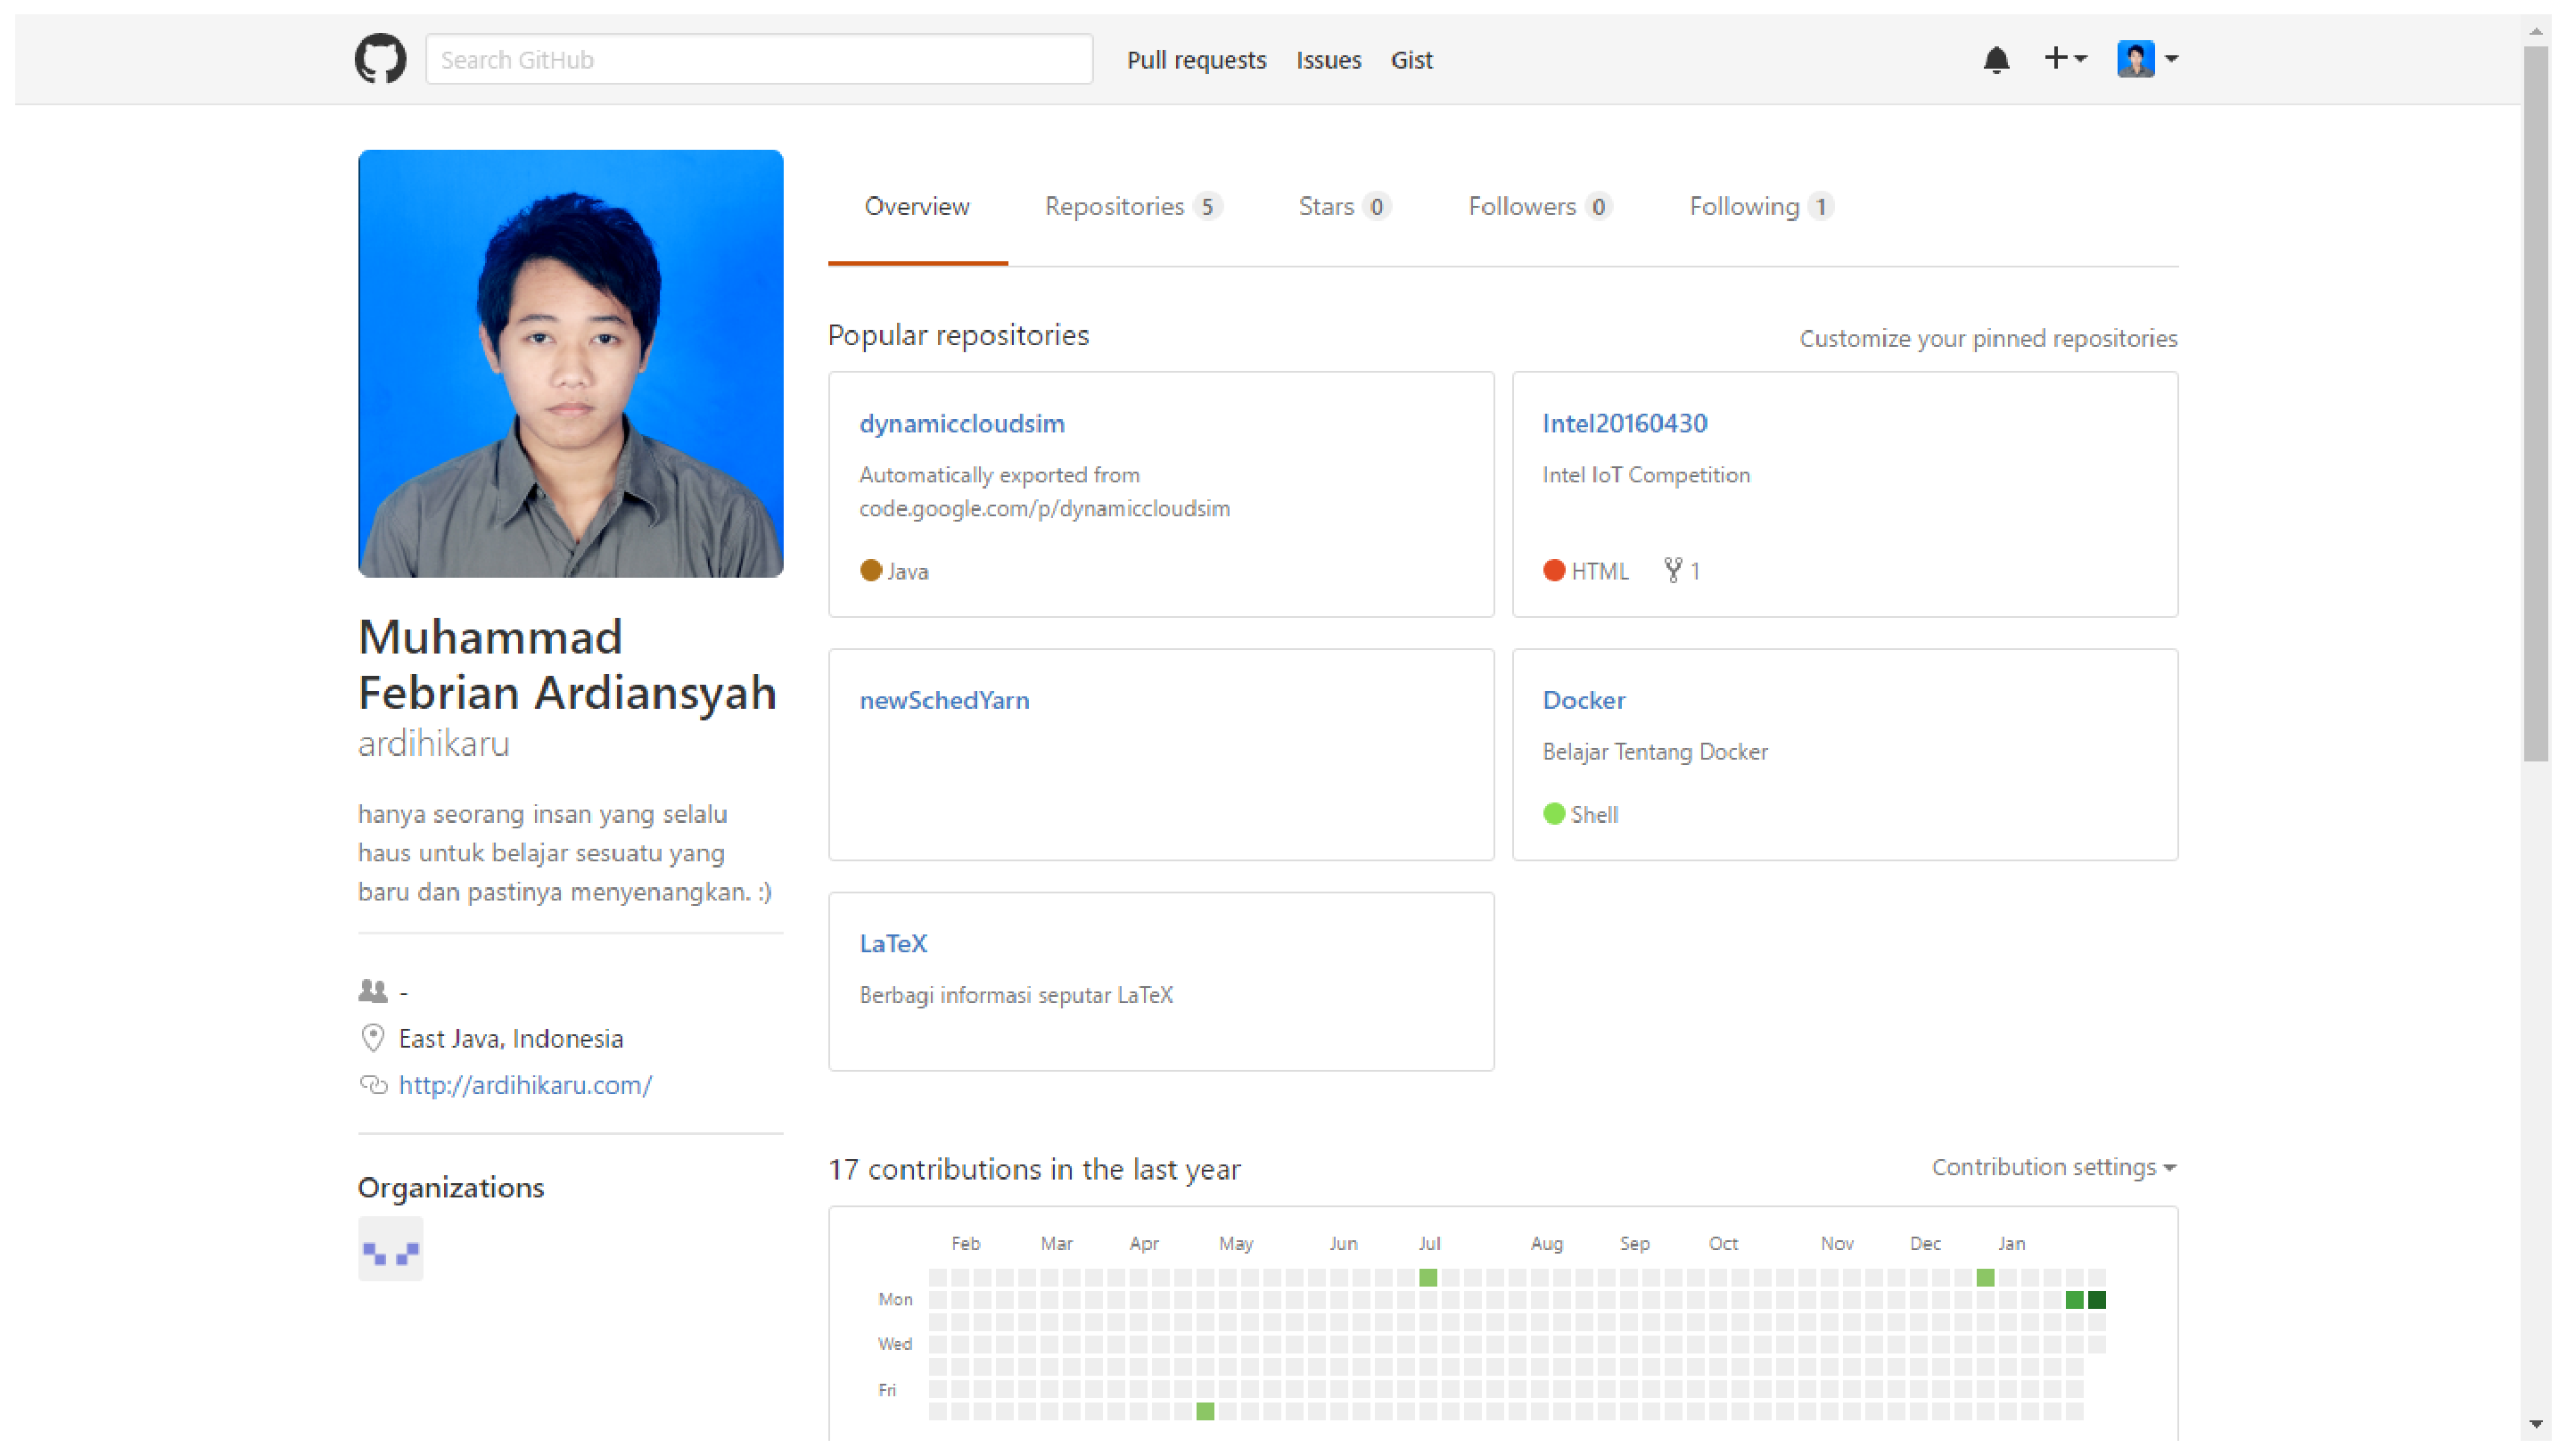
\includegraphics[width=\textwidth, keepaspectratio]{github}
%       \caption{Food choosing}
%       \label{fig:fig1a}
%   \end{subfigure}
%   \begin{subfigure}[b]{0.48\textwidth}
%       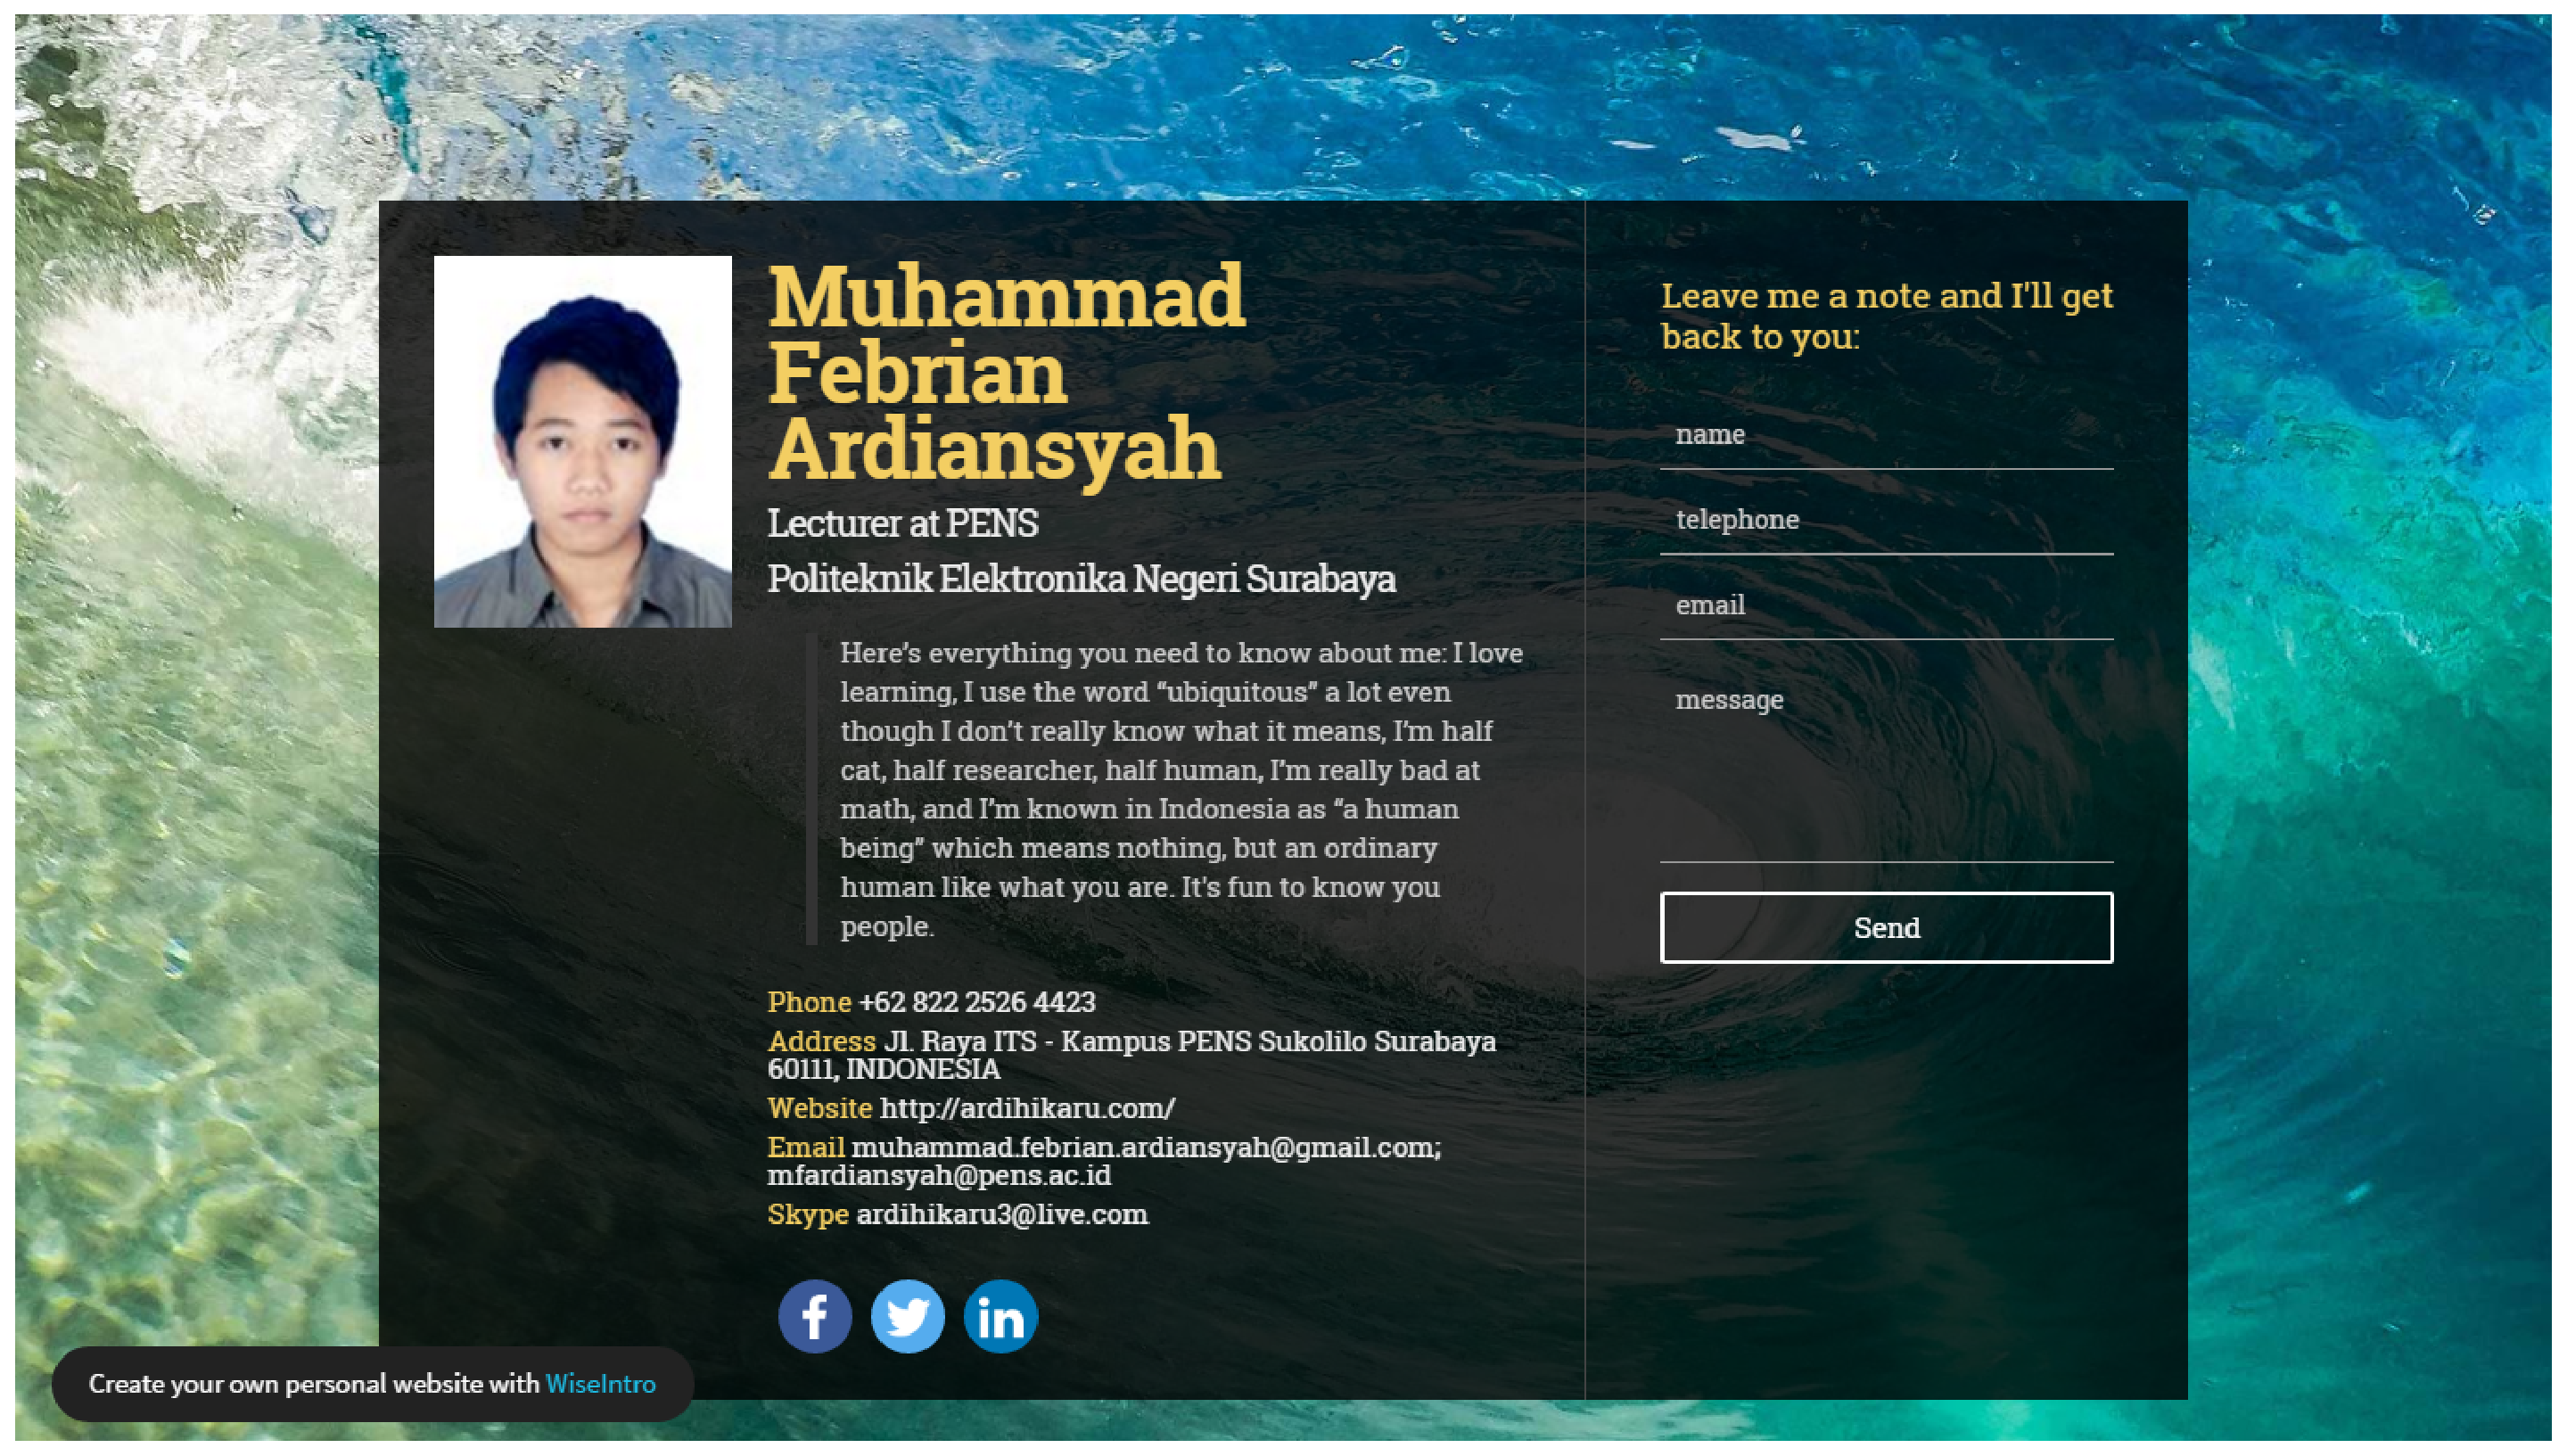
\includegraphics[width=\textwidth, keepaspectratio]{intro}
%       \caption{Interrelationship of different factors for different consumers}
%       \label{fig:fig1b}
%   \end{subfigure}
%   \caption{The difficulties of choosing food and its different adverse reactions}\label{fig1}
%\end{figure*}
%

\begin{figure}[H]
\centering
  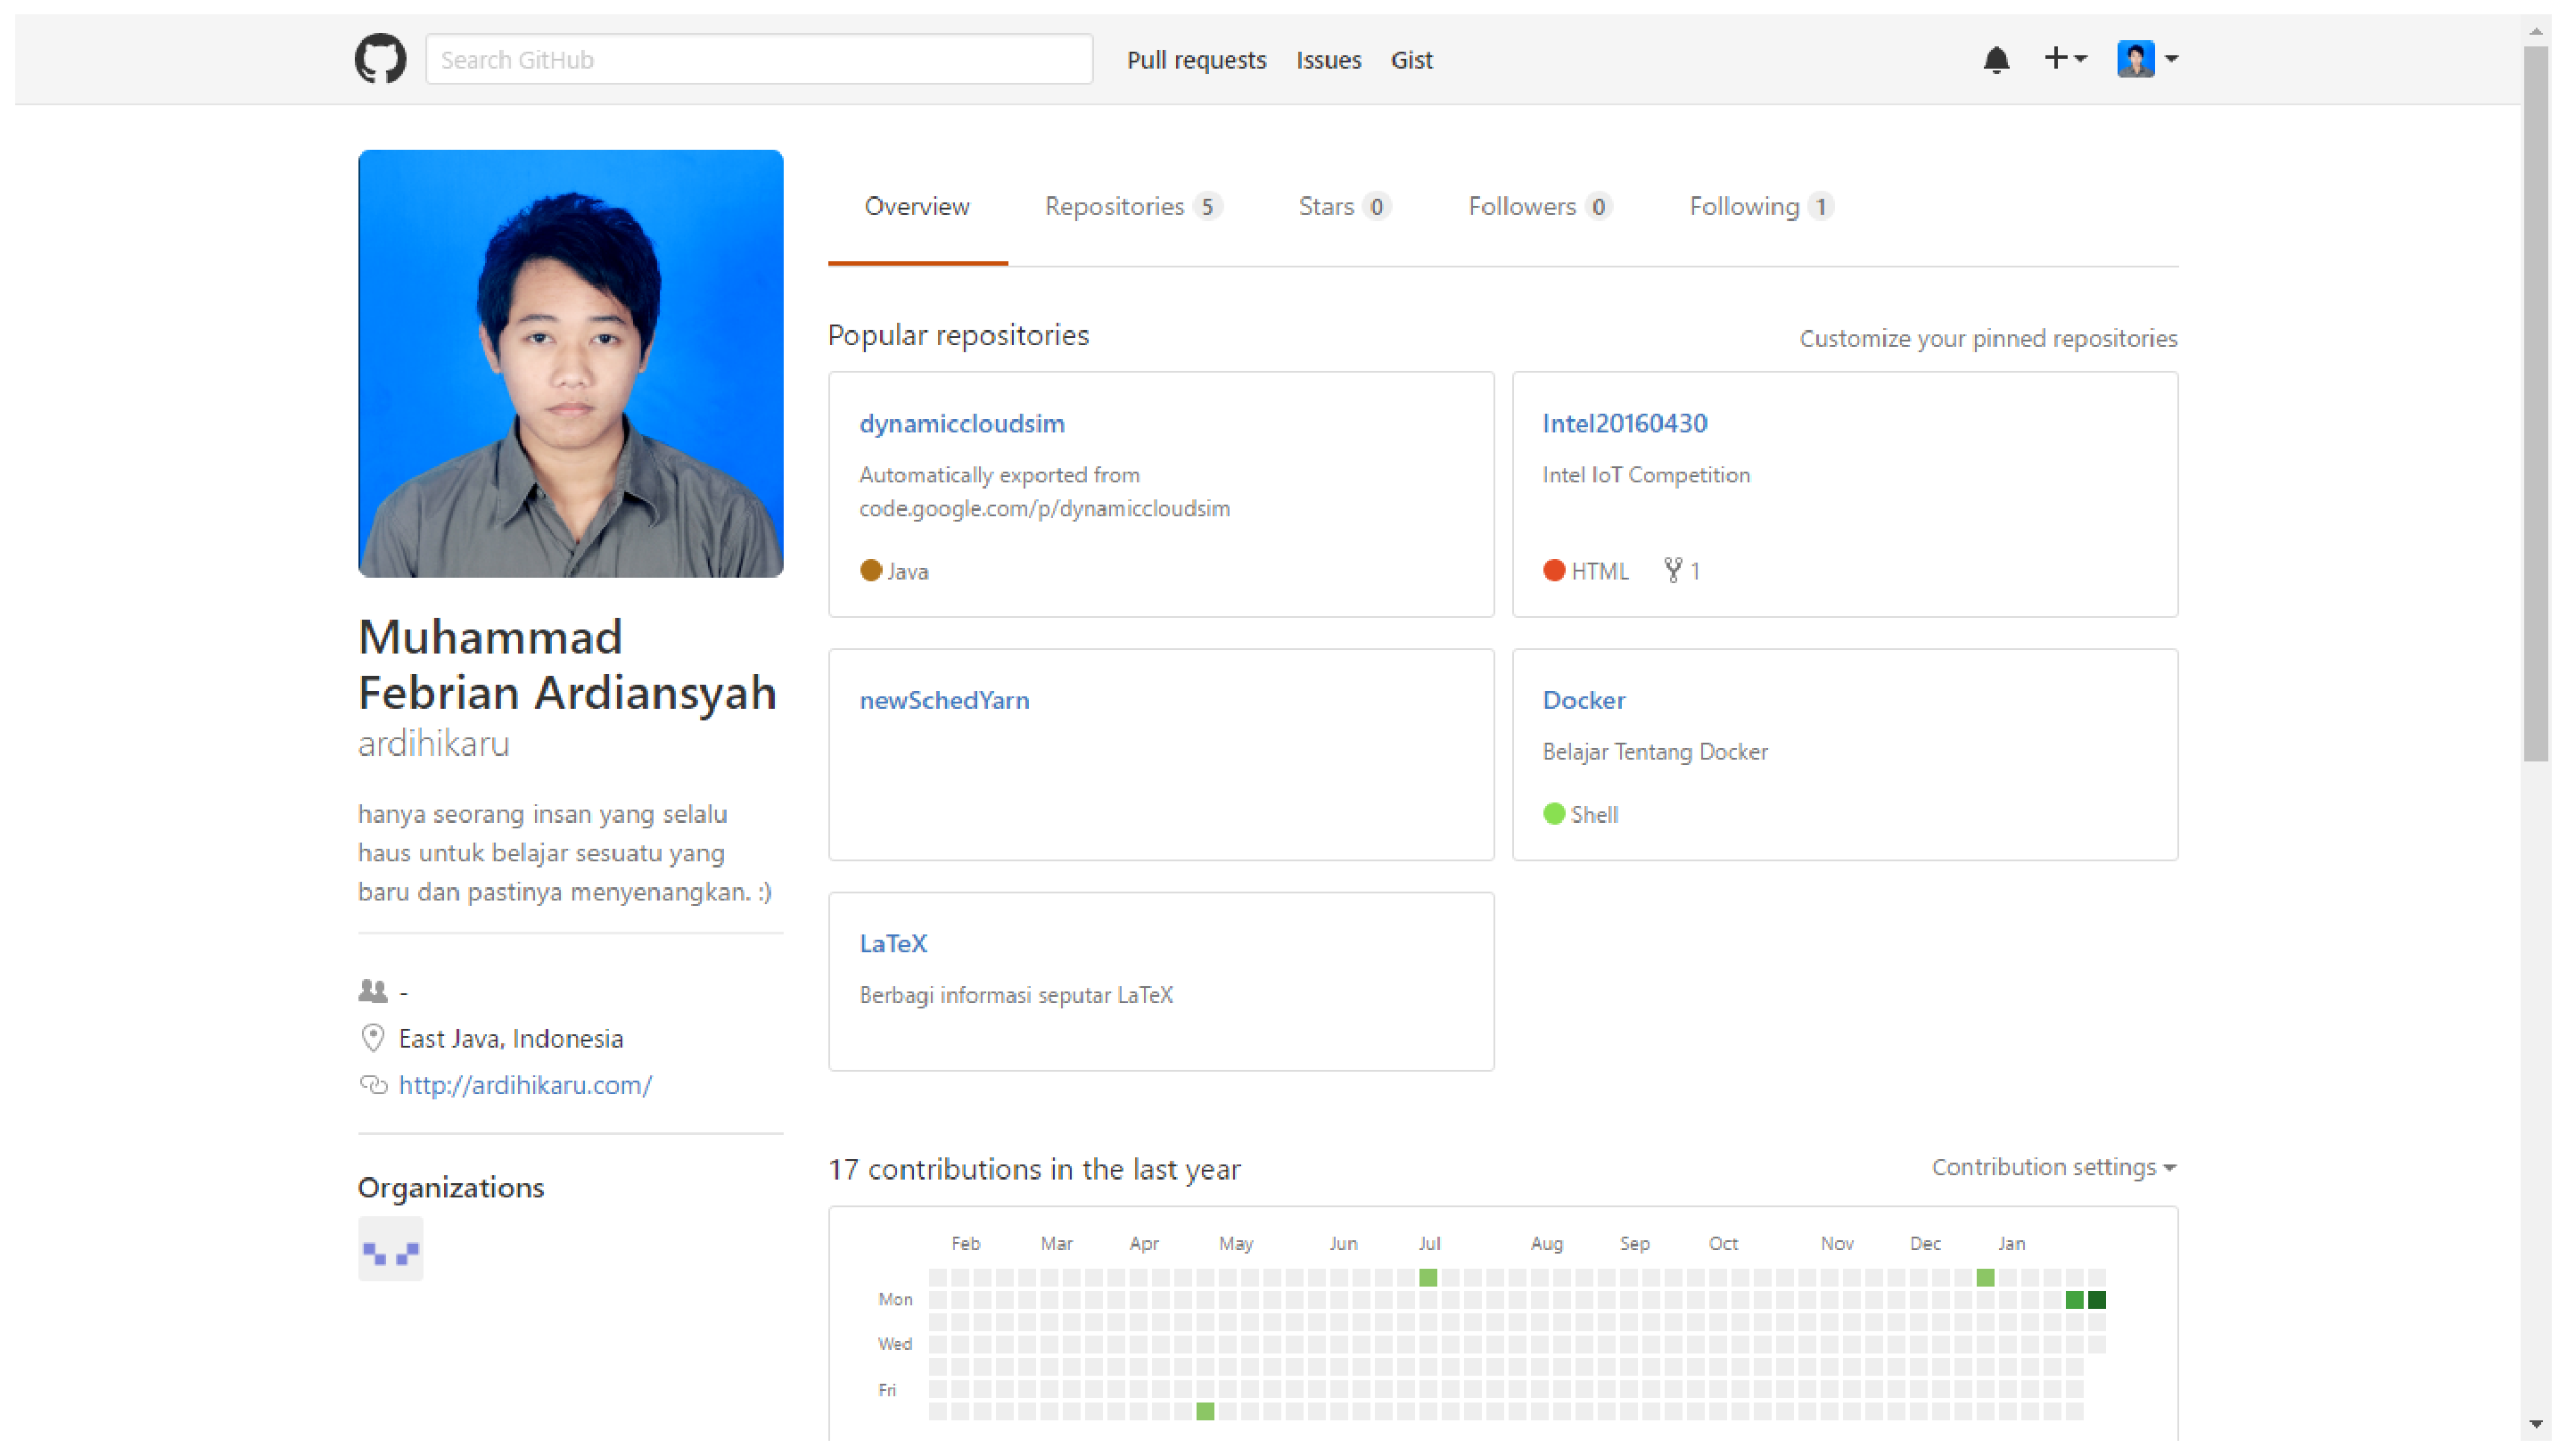
\includegraphics[width=0.35\textwidth]{github}
\caption{Intro}
\label{fig:fig1a}
\end{figure}

\begin{figure}[H]
\centering
  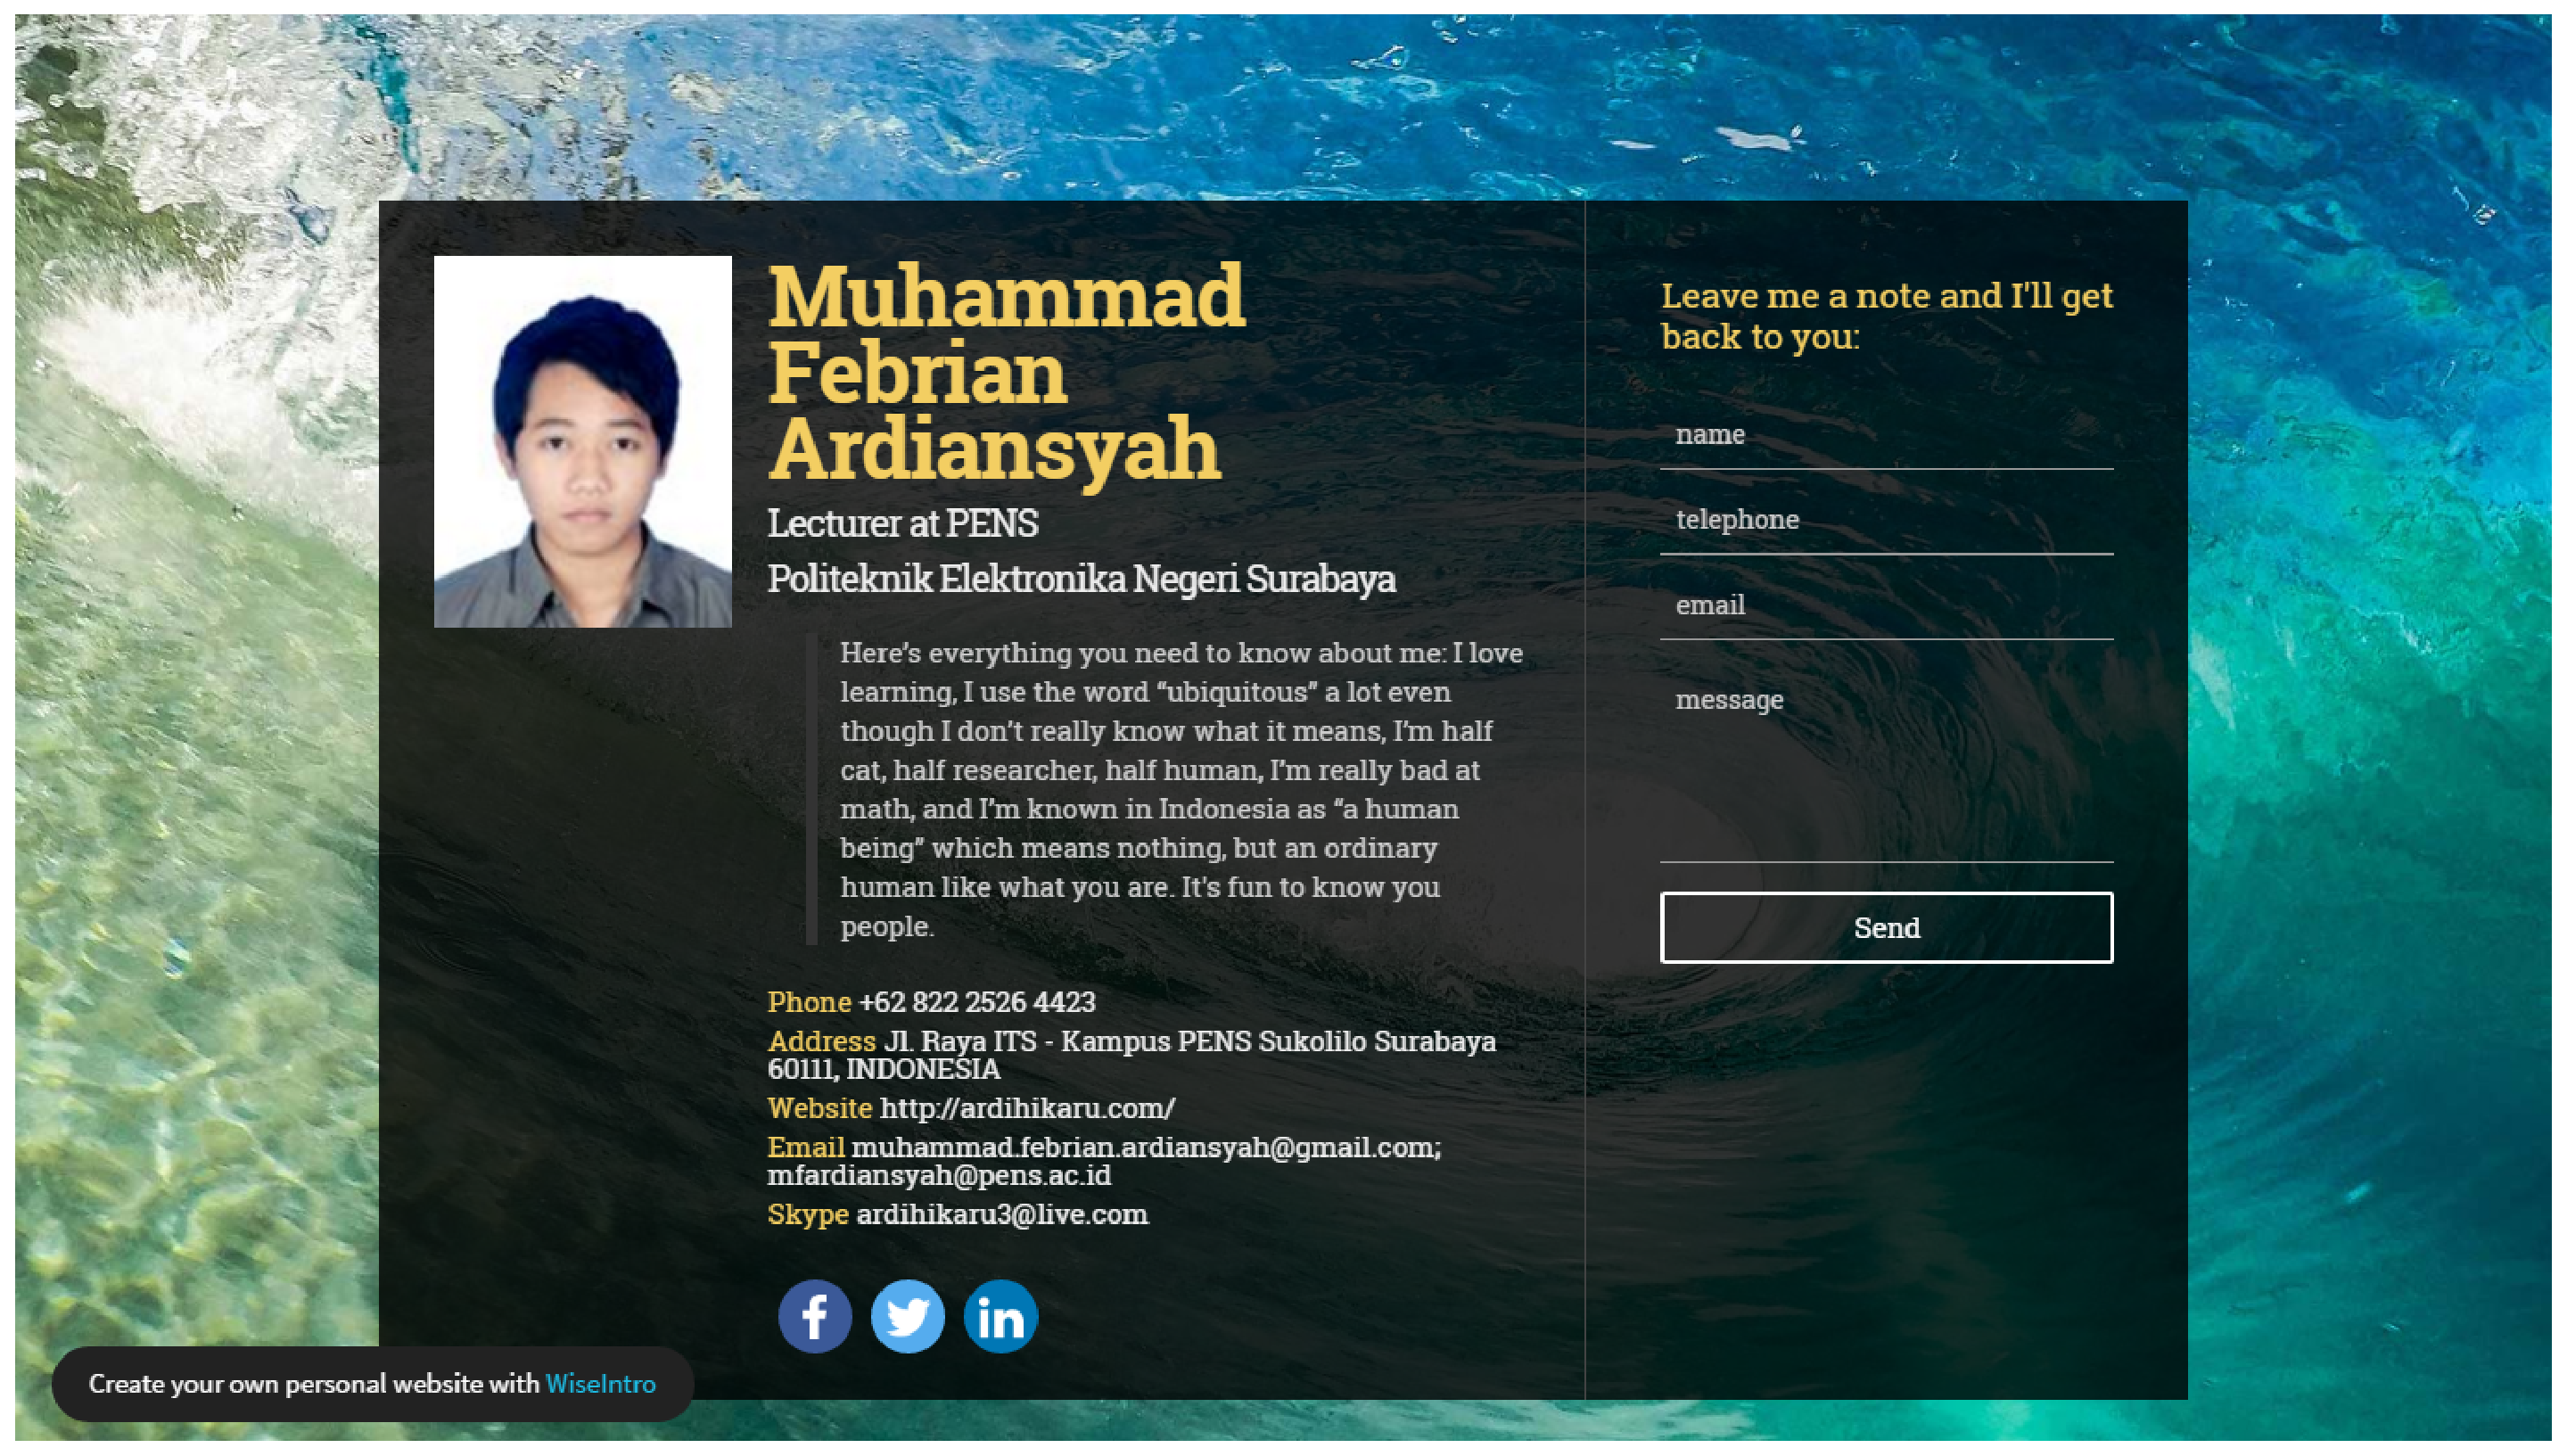
\includegraphics[width=0.35\textwidth]{intro}
\caption{Intro}
\label{fig:fig1b}
\end{figure}

\subsection{Name of the subsection 1: e.g. Using figures}
Subsection is here. In latex, it is suggested to use $.eps$ extension as our figure files. Do not ask me why, just trust me, it works! haha. Saran saya, gunakanlah ekstensi $.eps$ untuk gambar-gambar anda. Jangan ditanya ya, percaya saja. (Why? Google it yourself!). 

I use this $online tool$ \footnote{\label{note:eps_converter1}\url{http://www.tlhiv.org/rast2vec/}}. to convert my images into EPS format (resulted smaller and acceptable size). However, sometimes the webpage went offline. If you find some alternative sites, please fell free to share with me, with us.

Use $\backslash ref\{fig:fig1a\}$ (example: Fig.~\ref{fig:fig1a}) to show a figure. In Fig.~\ref{fig:fig1a}, it gives an example of a figure with multiple subfigures. Name $fig:fig1a$ is taken from figure's label. Syntax $\backslash ref\{fig:fig1a\}$ digunakan untuk menampilkan gambar yang sudah di-$attach$ di paper ini. Gambar Fig.~\ref{fig:fig1a} mencontohkan sebuah gambar dengan beberapa sub-gambar.

\begin{figure}[H]
\centering
  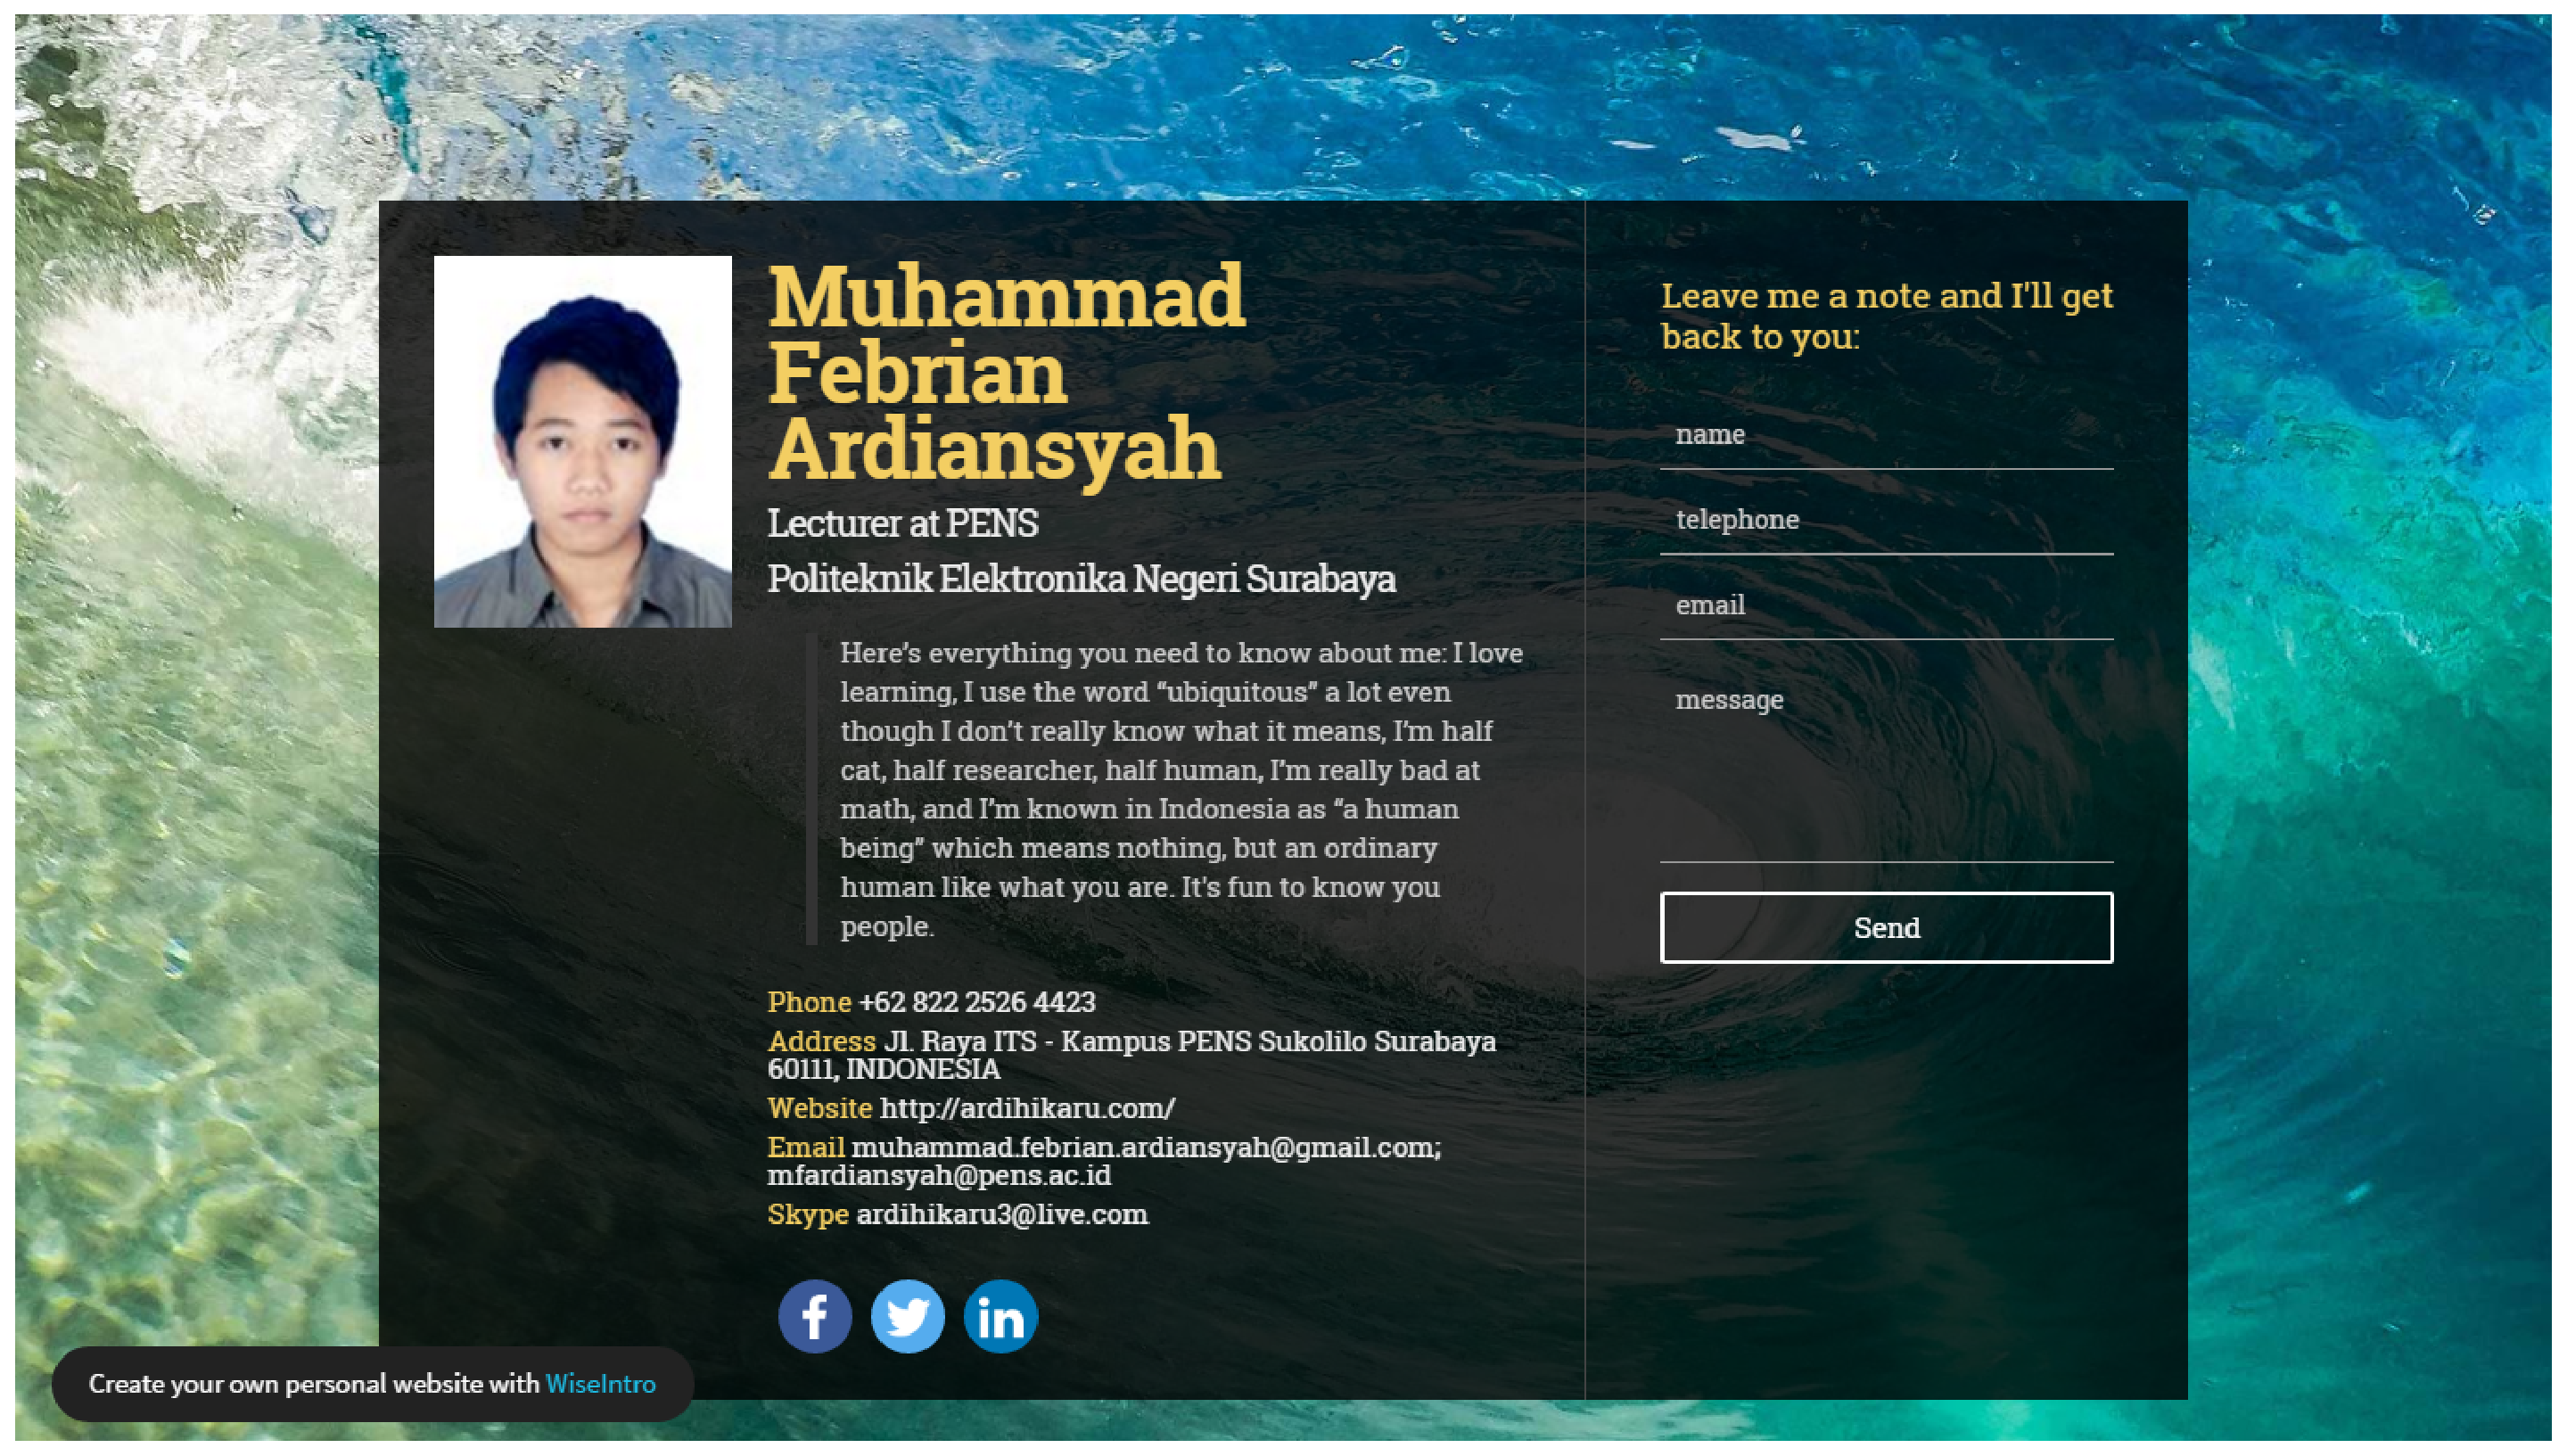
\includegraphics[width=0.35\textwidth]{intro}
\caption{Intro}
\label{fig:fig2}
\end{figure}

Here is another way plot a figure. Fig.~\ref{fig:fig2} is a single figure. There are many ways to plot figures. For the further information, you can check it into $Latex \lq s~wiki$ \footnote{\label{note:latex_wiki_figures}\url{https://en.wikibooks.org/wiki/LaTeX/Floats,_Figures_and_Captions}}. Berikut merupakan cara lain untuk menampilkan gambar. Fig.~\ref{fig:fig2} adalah contoh untuk menampilkan sebuah gambar. Untuk informasi lebih detail, silahkan merujuk $Latex \lq s~wiki$ \footnotemark[\ref{note:latex_wiki_figures}] (yang ini menggunakan rujukan $footnote$). 

Here you may find this itemizing useful.
\begin{itemize}
  \item Item 1.
  \item Item 2.
  \item Item 3.
\end{itemize}

End of introduction section. You may close it with a summary like this: \textquote{\textit{In the rest of this paper, the related works are reviewed in Section 2. Our proposed architecture and system model is discussed in Section 3. Section 4 discusses the methodology we are using our proposed architecture. Then, Section 5 evaluates our research study with some simulation results. Finally, Section 6 summarizes this paper}}. Lanjuutttt...

\section{Related Work}
Related works' here. Tuliskan related work disini.
    
\section{Another Section}

\subsection{Another Subsection 1}
Content goes here... 

\subsection{Another Subsection 2}
Content goes here... 

\subsection{Subsection 3: with subsubsection}

\subsection{Another Subsubsection 1}
Content goes here... 

\subsection{Another Subsubsection 2}
Content goes here... 

\section{Section Sample: Research Methodology}
In this section, we will ...

\subsection{Just Another Subsection} 
Let's discuss about $equation$.

\subsubsection{Just Another subsub: Equation example}
Example 1: BMI Formula \cite{nameofref1}. Syntax $\backslash ref\{eq:1\}$ (Example: \ref{eq:1}) is used to call the equation. Contoh 1: Rumus BMI \cite{nameofref1}. Silahkan gunakan syntax $\backslash ref\{eq:1\}$ (Contoh: \ref{eq:1}) untuk memanggil equation tersebut.

% BMI equation here
\begin{equation}‎
\label{eq:1}
BMI‎ ‎=‎ \frac {we} {he^2}
\end{equation}‎

In equation \ref{eq:2}, it gives another example of how to make use of this $equation$ syntax. Di equation \ref{eq:2} ditunjukkan bagaimana cara lain dalam penggunaan syntax ini.

\begin{equation}‎
\label{eq:2}
K(U, W, C) = 
\mathlarger{\mathlarger{‎‎\sum}}_{i=1}^{N‎}
\mathlarger{\mathlarger{‎‎\sum}}_{k=1}^{K}
\gamma_{ik} (\omega_\alpha \times \omega_\beta)_{x_i} D(x_i,c_k)
\end{equation}‎

For further usage, this $reference$ \footnote{\label{note:latex_wiki_math}\url{https://en.wikibooks.org/wiki/LaTeX/Mathematics}} or $this~one$ \footnote{\label{note:latex_wiki_advmath}\url{https://en.wikibooks.org/wiki/LaTeX/Advanced_Mathematics}} might help you. Untuk informasi lebih detail tentang $equation$, silahkan merujuk ke $sini$ \footnotemark[\ref{note:latex_wiki_math}] atau ke $sana$ \footnotemark[\ref{note:latex_wiki_advmath}].

\subsubsection{Just Another subsub: Algorithm example}
Let's go through how do we write an algorithm and how to $summon$ it into our masterpiece! Berikut merupakan cara penulisan algoritma dan pemanggilannya.

\begin{algorithm}[H]
  \caption{Name of the algorithm, contoh: Algojlo untuk pengguna $U$}
  \label{alg:1}
  \begin{algorithmic}[1]
    \Require
      \Statex Data Matrik (A, B) $a \times b \to \phi \times y$.
      \Statex Titik datanya $pn = \{p_1, xp_2, ..., p_l\}$; 
      			$~p_i \to namafunc(x,y) = xxx \times yyy$\
      \Statex Set $G$ untuk percobaan.
      
    \Ensure
      \Statex (Pastikan) setiap var $p_i$ berjodoh (ehem) dengan $gueh$.
	
	\Statex
	
	\State Bangkitkan var $P$ acak acak acakkkkk;
    \For  {$i=1$ to $g$} 
    	\For  {$k=1$ to $r$} 
    		\State Hitung $Rumus 1$; 
    		\State Tanya $Rumus 2$; \Comment{(tanya ken, apa?)}
    		\State Tinggalkan $Rumus 3$;   
    	\EndFor   
    \EndFor  
    %%%
    \For  {$i=1$ to $g$} 
    	\For  {$k=1$ to $r$} 
    		\State Hitung $Rumus 1$; 
    		\State Tanya $Rumus 2$; \Comment{(tanya ken, apa?)}
    		\State Tinggalkan $Rumus 3$;   
    	\EndFor   
    \EndFor  
    %%%
    \State Samakan $a = a$;
    \For  {$k=1$ to $D$} 
    	\State Makan ${roti}^{isi}_{misis}$; 
    	\If {$y_{coba(baru)} \neq g^{dor}$}
    		\State Lewati;
		\EndIf
    \EndFor   
    \State Return $y$;
    %%%
    \If {$lanjut(true)$}
    	\State Kembali ke $line~6$;
	\EndIf
    
  \end{algorithmic}
\end{algorithm}

Penggilan algoritma bisa menggunakan: $\backslash ref\{alg:1\}$, contoh: \ref{alg:1}.

Contoh equation di paragraf: $\alpha_{coba} = \mathlarger{\mathlarger{‎‎\sum}}_{x=1}^{A‎} b^{cd}_e$, bisa juga $\alpha_{min} = MIN(\alpha)$ and $\alpha_{max} = MAX(\alpha)$. Gunakan $\{<<code here..>>\}$ jika variabel berupa kata.

\subsubsection{Just Another subsub: Table example}
Check it out!

\begin{table}[H]
\centering

\begin{tabular}{ |l|r|c| }
\hline
%\multicolumn{3}{ |c| }{Simulation Parameters} \\
%\hline

{Colomn 1} & \multicolumn{2}{ |c| }{Colomn 2 - multi-comlomn} \\ 
\hline %header

\multirow{3}{*}{Var 1 (3)} & 1.000 & \multirow{3}{*}{Detil var 1} \\
 & 2.000 & \\
 & 3.000 & \\ \hline
 
{Var 2} & 10 & {Type of Food} \\ \hline
 
\multirow{5}{*}{Var 3 (5)} & 2 & \multirow{5}{*}{Detil var 2} \\
 & 2 & \\
 & 4 & \\
 & 6 & \\
 & 8 & \\ \hline
 
\multirow{3}{*}{Var 4 (3)} & 10 & \multirow{3}{*}{Detil var 3} \\
 & 20 & \\
 & 30 & \\ \hline
 
\hline
\end{tabular}

\caption{Contoh tabel}
\label{table:example}
\end{table}

Penggilan tabel bisa menggunakan: $\backslash ref\{table:example\}$, contoh: \ref{table:example}.

\subsubsection{Just Another subsub: How to find reference}
You can try using $google scholar$ \footnote{\label{note:google_scholar}\url{https://scholar.google.co.id/}} to get the bib script. Follow this step-by-step from Figures \ref{fig:fig3_1}, \ref{fig:fig3_2}, \ref{fig:fig3_3}, \ref{fig:fig3_4} below.

\begin{figure}[H]
\centering
  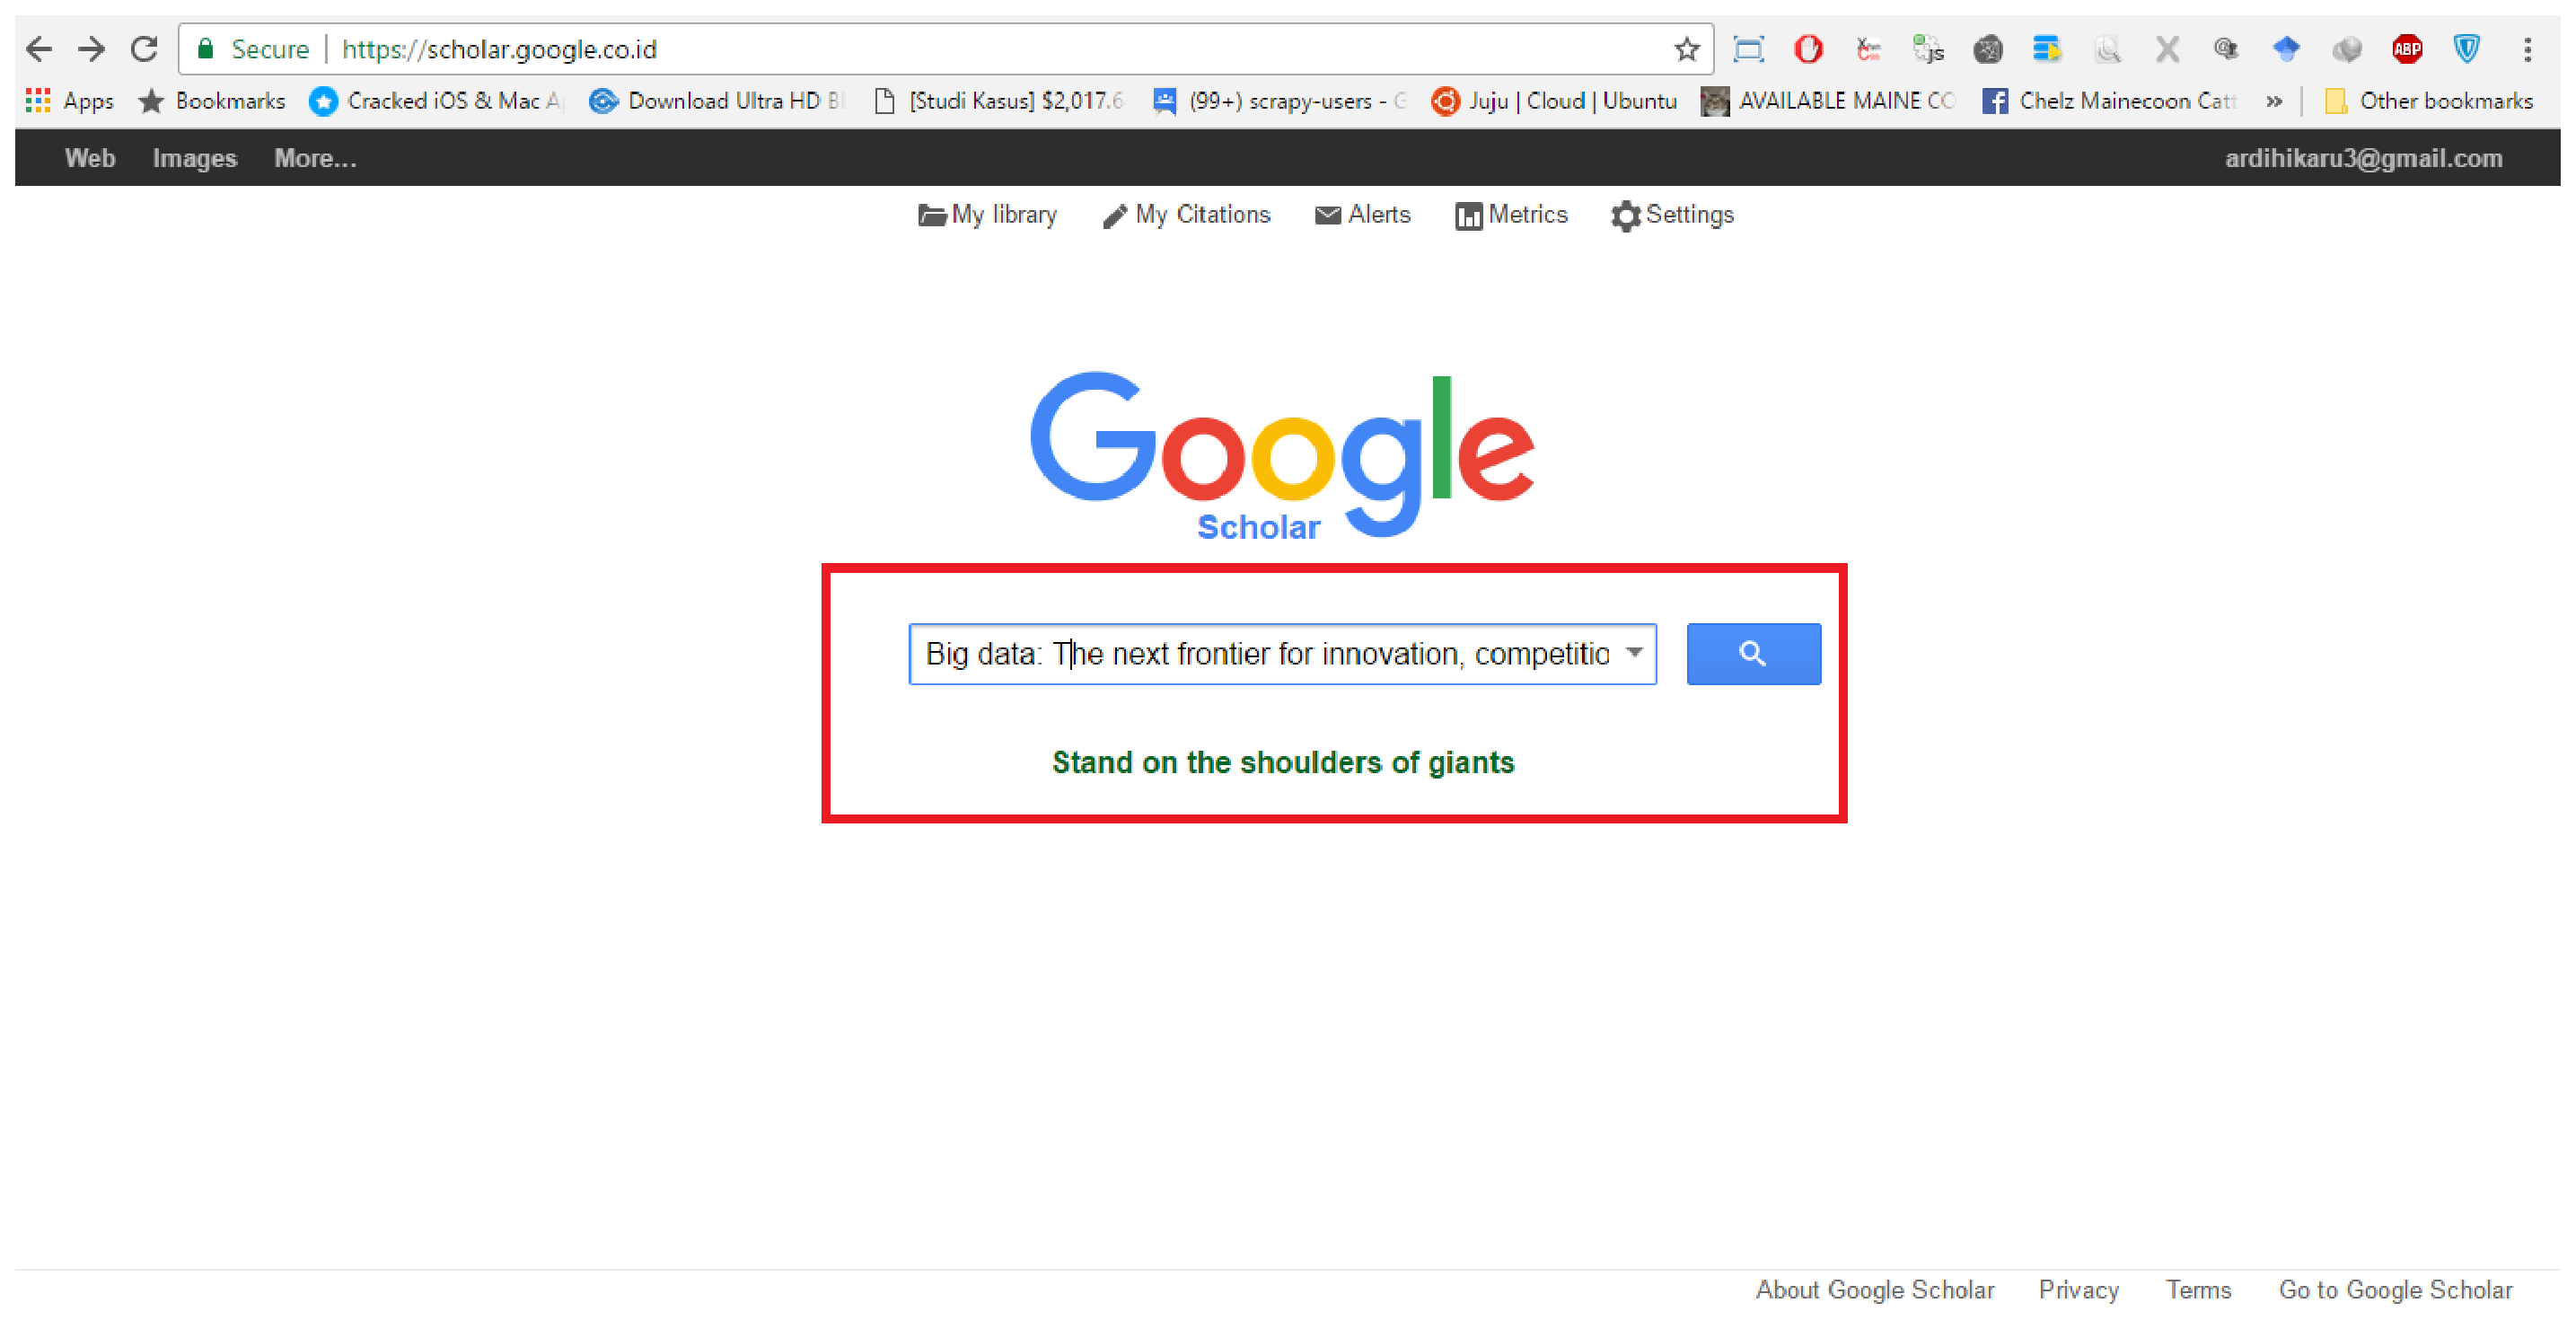
\includegraphics[width=0.35\textwidth]{get_bib_script_part_1}
\caption{Buka Google Scholar}
\label{fig:fig3_1}
\end{figure}

\begin{figure}[H]
\centering
  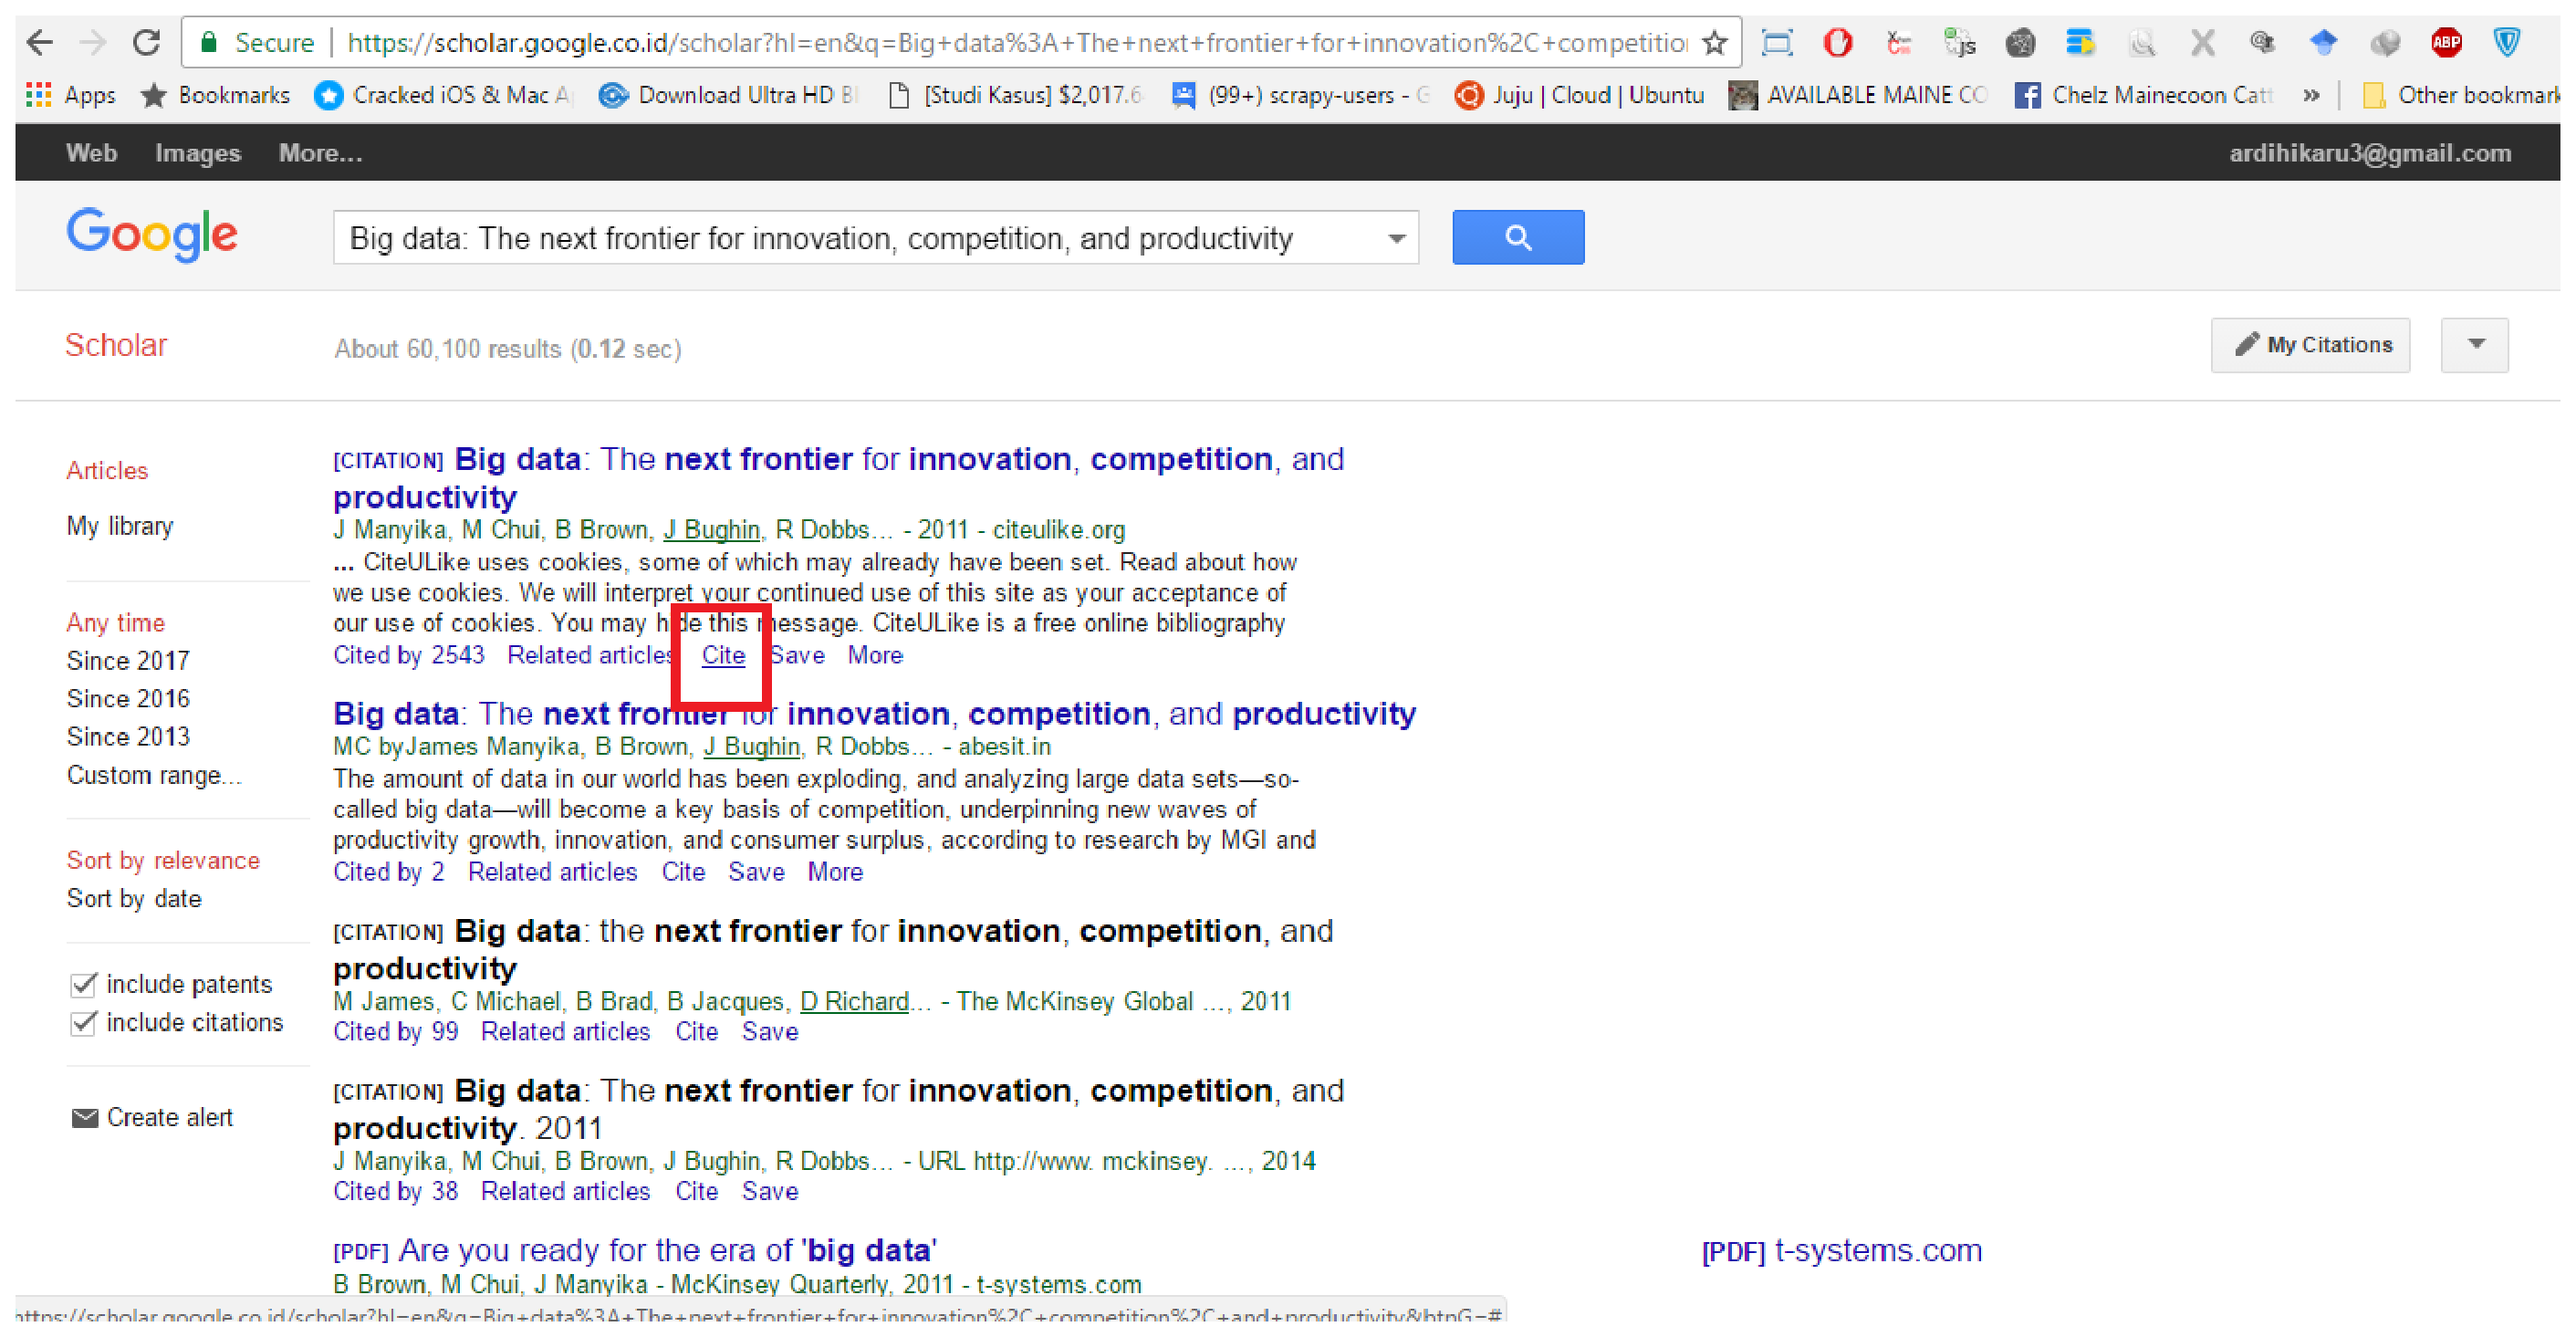
\includegraphics[width=0.35\textwidth]{get_bib_script_part_2}
\caption{Click of the $Cite$ link.}
\label{fig:fig3_2}
\end{figure}

\begin{figure}[H]
\centering
  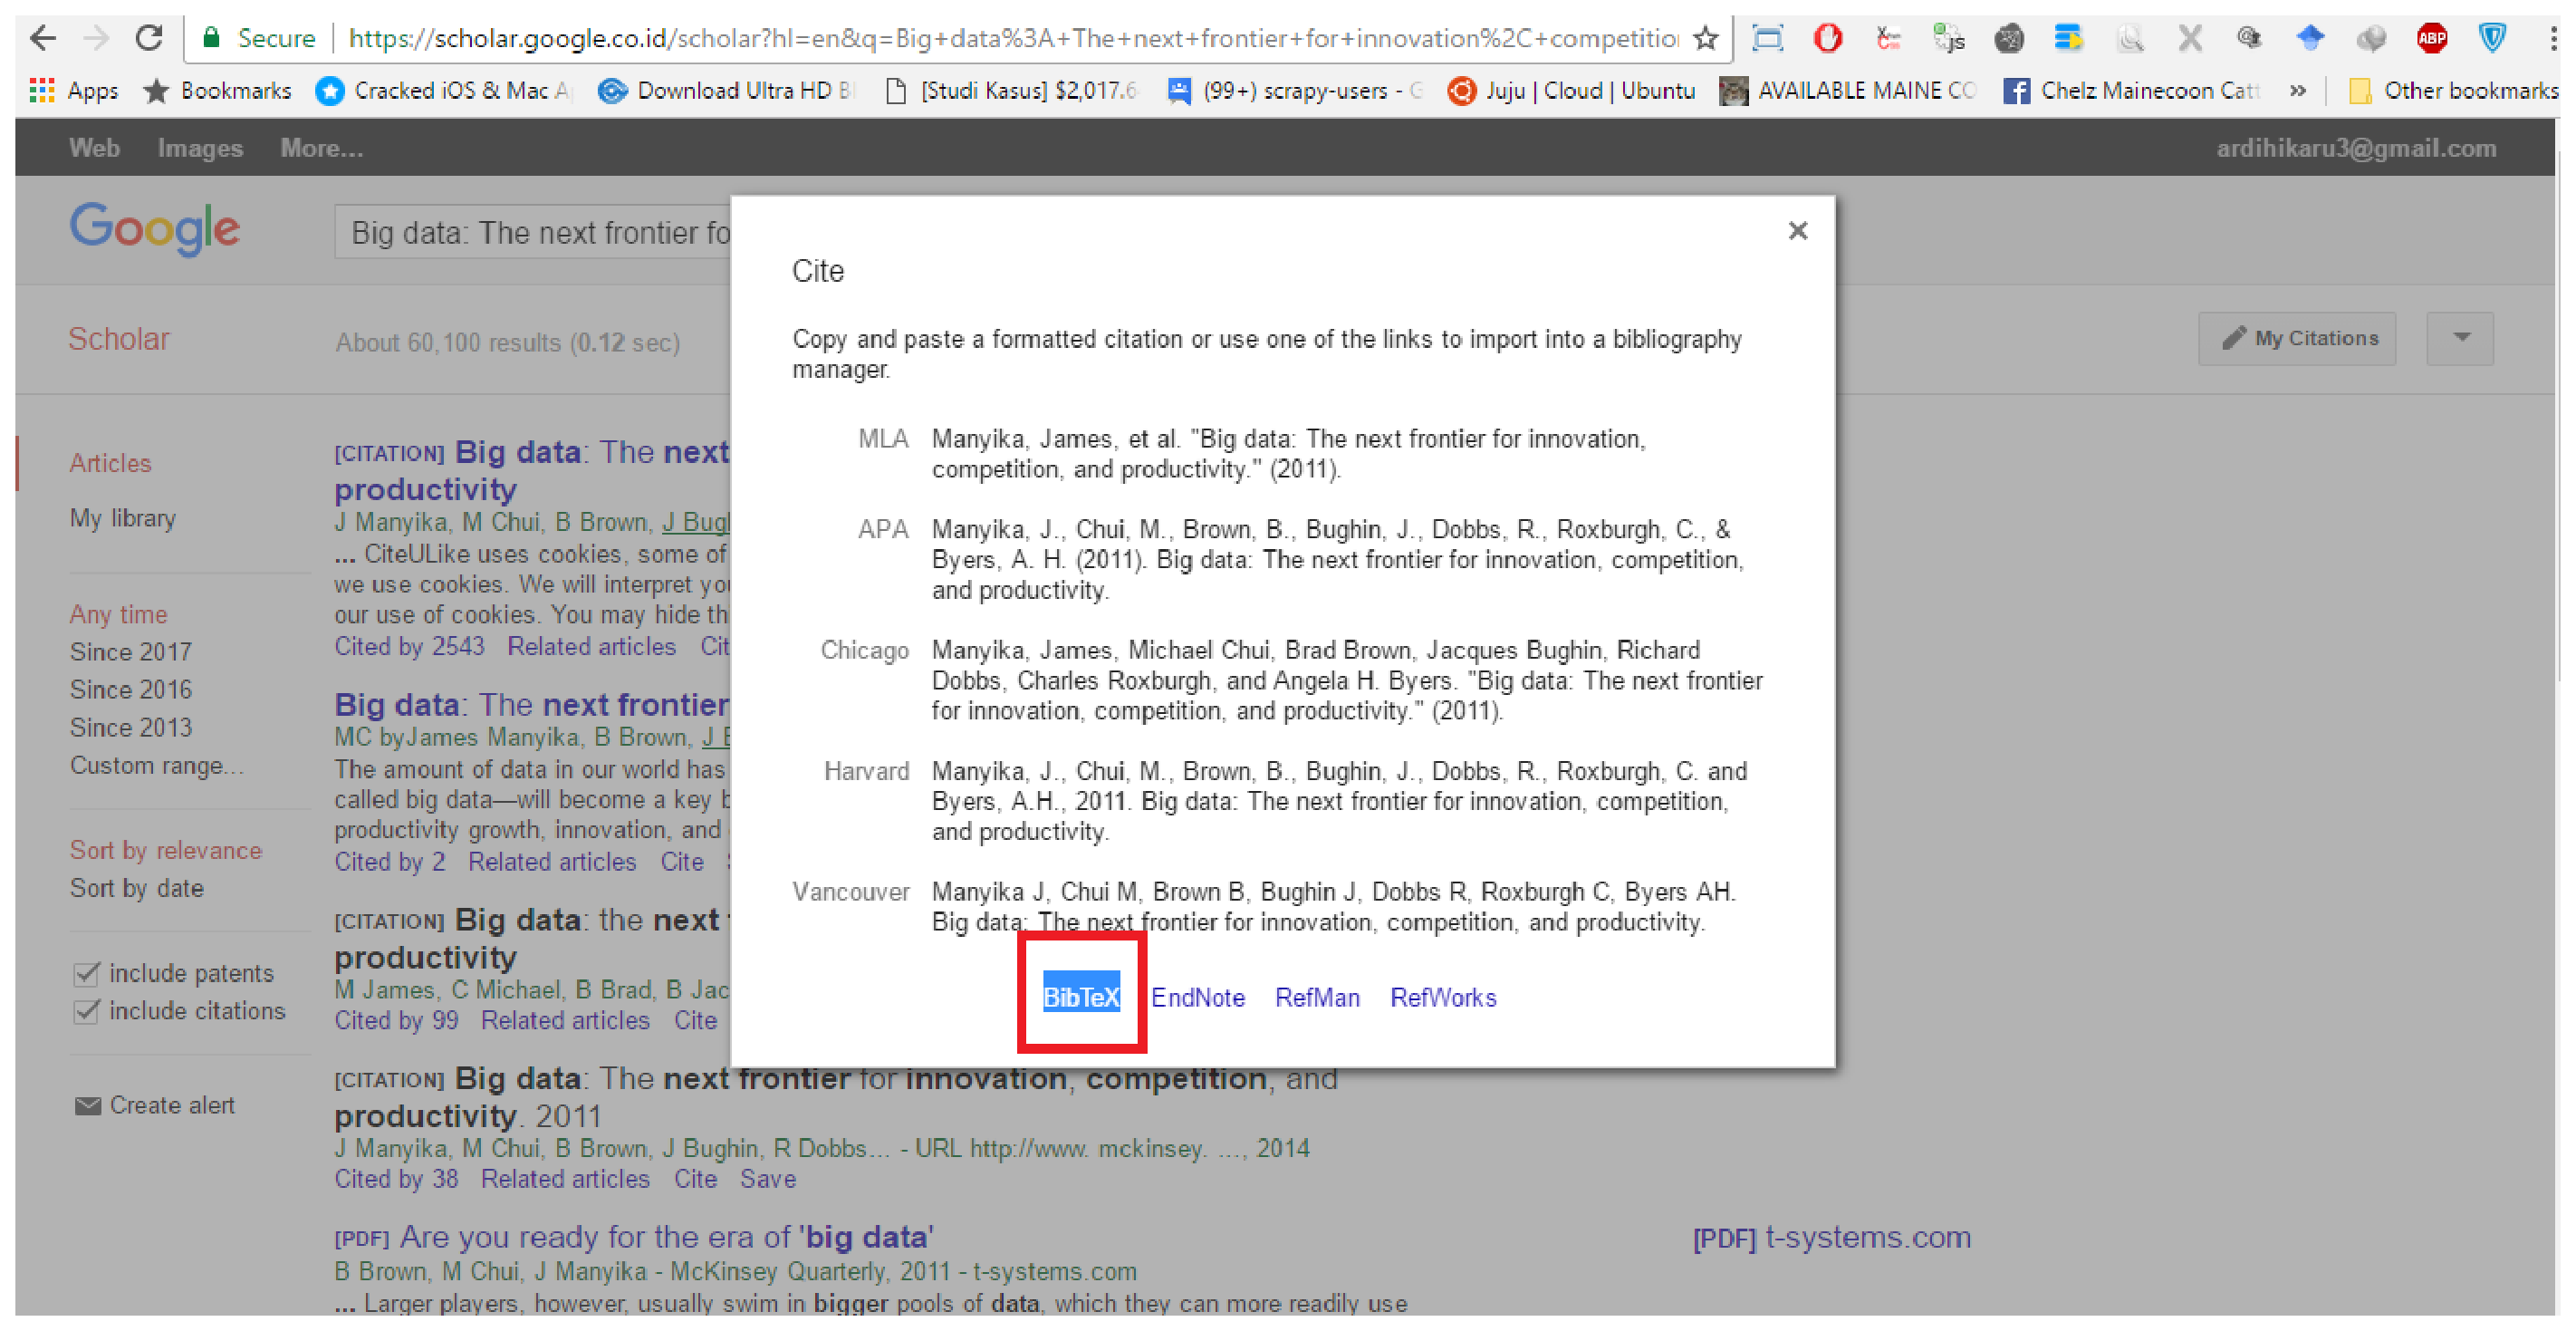
\includegraphics[width=0.35\textwidth]{get_bib_script_part_3}
\caption{Click of the $BibTeX$ link.}
\label{fig:fig3_3}
\end{figure}

\begin{figure}[H]
\centering
  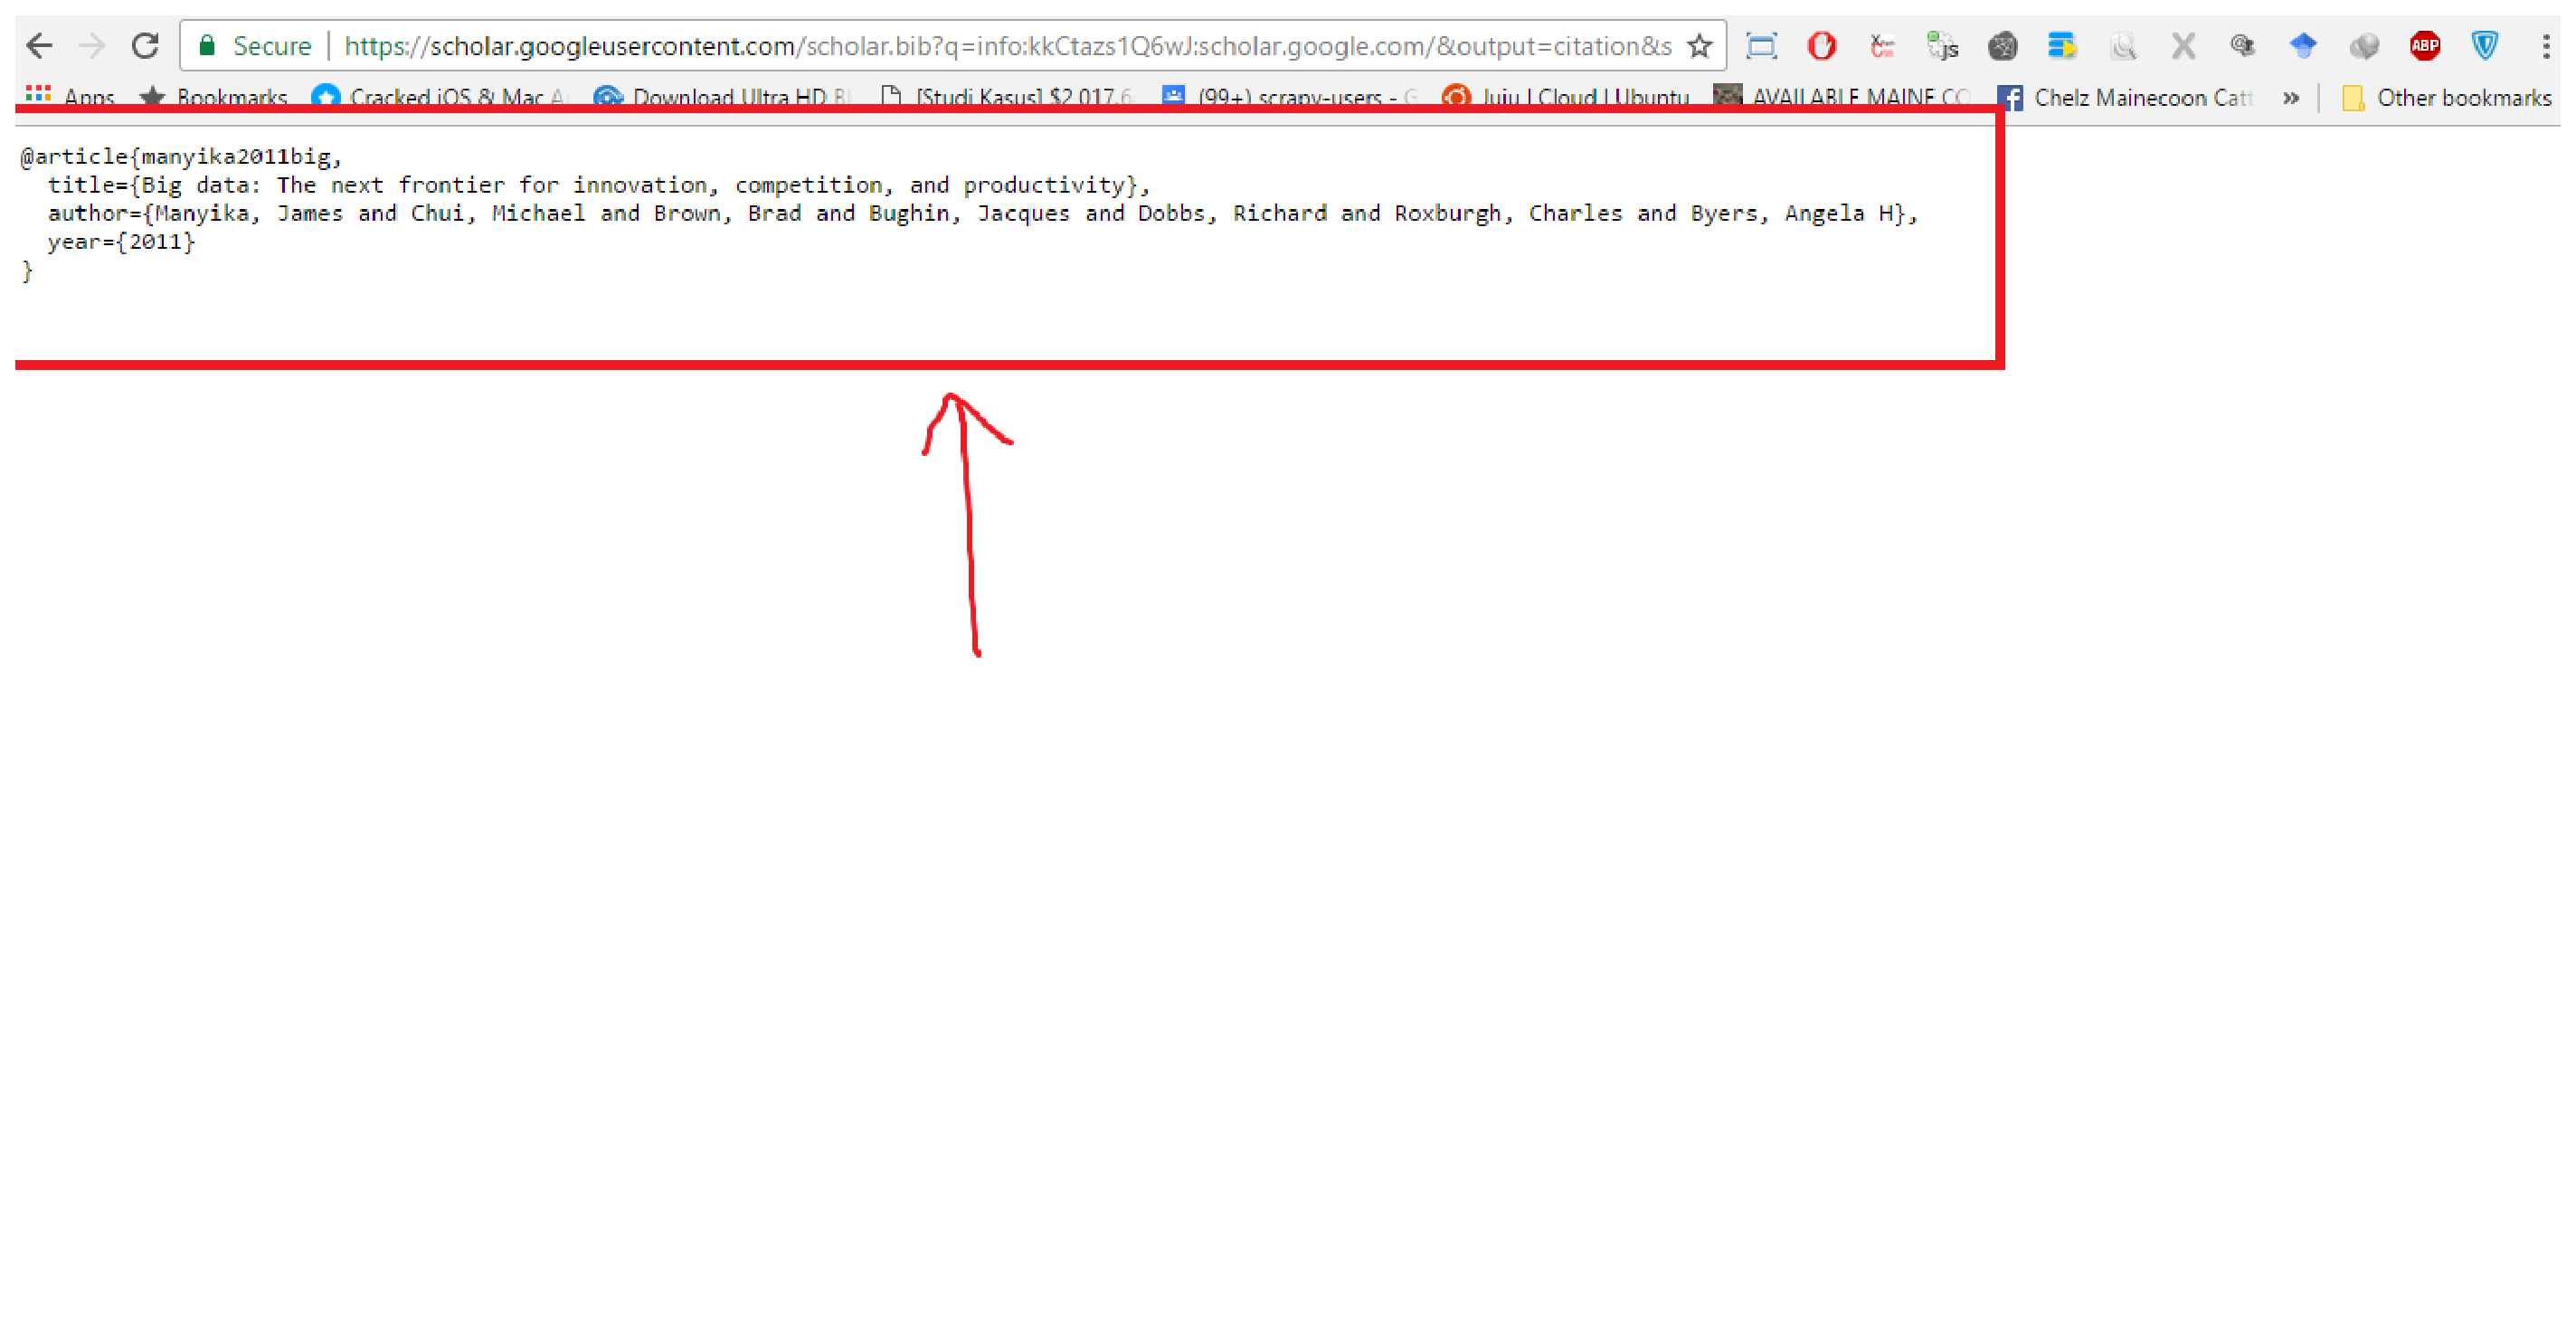
\includegraphics[width=0.35\textwidth]{get_bib_script_part_4}
\caption{Copy the text}
\label{fig:fig3_4}
\end{figure}

For URL type references, you may check on one of my example of the $mybib.bib$ file. Once again, there are lots of alternative ways to write in LaTeX file. 

\section{Simulation}
Content goes here... 

\subsection{Simulation Setup}
Content goes here... 

\subsection{Simulation Results}
Content goes here... 

\section{Conclusion}
Content goes here... 

See you again, hopefully it is useful for you guys! enjoy!

\appendices
\section{Proof of the First Zonklar Equation}
Appendix one text goes here.

\section{}
Appendix two text goes here.

% use section* for acknowledgment
\section*{Acknowledgment}

The authors would like to thank...

% Can use something like this to put references on a page
% by themselves when using endfloat and the captionsoff option.
\ifCLASSOPTIONcaptionsoff
  \newpage
\fi

\bibliographystyle{unsrt}   % this means that the order of references
\bibliography{mybib}  % list here all the bibliographies that

\begin{IEEEbiography}{Author 1}
Biography text here.
\end{IEEEbiography}

\begin{IEEEbiography}{Author 2}
Biography text here.
\end{IEEEbiography}

% that's all folks
\end{document}


